\section{Protocols, samples, and statistical interpretation}
\label{app:methods}
The original experiments, the layout intervention, the bounded cap diagnostic, and the final studies retain their separate frozen designs. Local timestamped freezes precede each follow-up's evaluation outputs; they are not independently registered preregistrations. Development, smoke, historical legacy, and systems-timing outputs do not enter held-out task estimates.

\begin{table}[ht]
\centering\small
\caption{Evaluation inventory. Outputs are executions of conditions, not independent samples. The cap diagnostic is conditional on the original capped subset.}
\begin{tabular}{lrrl}\toprule
Study & Cases & Outputs & Independent unit\\\midrule
LoCoMo & 500 questions & 9,000 & 10 conversations\\
RULER-derived & 180 & 2,160 & Case, stratified by task\\
Original identifiers & 96 & 2,016 & Case, balanced factor design\\
Layout intervention & 48 & 576 & Paired held-out case\\
Controlled scale & 32 & 288 & Paired triplet\\
Fixed-budget retrieval & 30 base cases & 540 & Base case across lengths\\
Compact static storage & \nval{compact.n} & \nval{compact.calls} & Paired source triplet\\
LoCoMo cap sensitivity & 247 capped questions & 247 & Original conversation\\
Systems profiling & 1 source per length & 585 & Repeated invocation\\\bottomrule
\end{tabular}
\end{table}

The original study contributes 13,176 outputs. The layout intervention additionally uses 36 development calls on 12 cases, excluded from held-out estimates. The final round contributes 828 quality outputs and 585 profiling invocations, of which 135 are warmups and 450 are measured. The profiling instrumentation observes 585 top-level model forwards. This count does not measure internal forward calls of the quality runs or count their outputs as additional accuracy samples. The later compact-storage follow-up contributes \nval{compact.calls} additional quality outputs on \nval{compact.n} independent sources; its three answer-blind development sources and separate smoke cases do not enter estimates.

\paragraph{Decoding and scoring.}
The original LoCoMo, RULER-derived, and identifier caps are 96, 128, and 64 generated tokens, respectively. Both earlier final quality studies and the compact-storage follow-up use 64. Generation is greedy, with thinking disabled where the native interface supports that setting. The final studies use BF16, SDPA, batch one, and the inherited model generation configuration; the complete configuration accompanies each output. Token IDs are preserved as well as decoded text. Canonical identifier EM uses the frozen scorer's whitespace and answer normalization; it does not strip arbitrary prose to rescue an otherwise incorrect output. CER can exceed one when extra predicted characters outnumber reference characters. Literal-raw EM is a separate diagnostic because model-specific output wrappers can differ from the canonical answer.

\paragraph{Families and intervals.}
The original confirmatory family consists of three directional LoCoMo package tests and three original identifier contrasts. Its six-test Holm correction is retained. For LoCoMo H1, the statistic is the mean of ten paired conversation-level F1 differences, selected optical minus full optical. The one-sided upper-tail test enumerates all sign assignments, conditions on the observed magnitudes, and assumes sign symmetry under the null; condition assignment was not randomized. The LoCoMo same-evidence comparison estimates a difference and assesses a prespecified equivalence margin; it is not silently added as a new directional discovery. The RULER sweep is descriptive. Layout uses three two-sided exact McNemar tests in its own Holm family. Scale uses three exact conditional omnibus tests, with nine pairwise secondary tests in a separate family. Fixed-budget retrieval uses three primary interaction tests and a separate family of three secondary LONG tests. The compact-storage follow-up has one confirmatory optical--compact McNemar contrast, with other arm and position comparisons descriptive. There is no single global correction across these prospectively separated studies.

Paired percentile bootstrap intervals use 50,000 resamples. LoCoMo resamples whole conversations with equal weight, not individual questions. RULER resampling is stratified by task and keeps a case's representations together. Layout resampling is stratified within its 24 two-instance cells. With only two cases per cell, these intervals warrant caution: cells with identical observed differences contribute no bootstrap variation. The exact paired tests provide the confirmatory layout evidence. Scale and the original fixed-budget study resample paired cases; the compact-storage follow-up resamples paired triplets within its three position strata. These intervals are pointwise. Boundary intervals from zero successes or zero observed differences do not imply population certainty. Cluster sign tests and $t$ intervals below are sensitivity analyses, not additional confirmatory tests.

\section{Dialogue memory: complete comparisons and cap sensitivity}
\label{app:locomo}
The LoCoMo subset comprises the recorded 500 questions in ten previously studied conversation clusters, with 105, 108, and 287 questions in categories 1, 2, and 4. Expansion of question coverage does not create new independent conversations. We preserve dated chronological memories, speaker and turn identifiers, text, and shared-image captions. The BM25 retriever uses $k_1=1.5$, $b=0.75$, lowercase ASCII alphanumeric terms, and stable source-index tie-breaking. It selects the top 16 turns within the question's conversation and restores source order. It never uses reference answers, evidence annotations, or reader scores.

The same-evidence text and optical conditions receive identical canonical strings and turn metadata. Retrieved optical uses a single 1,372-pixel square RGB page, an 8-pixel source font, and 24-pixel margins. Full optical is calibrated to approximately $C=2$. The full-optical-budget text control greedily packs whole turns using the same ranking and skips oversized turns. The selected-optical-budget text control uses the frozen ranked-prefix rule without splitting turns or skipping an earlier ranked turn. These controls share a budget with their optical counterpart, not necessarily the same evidence.

\begin{table}[ht]\centering\small
\caption{All principal LoCoMo paired differences, in F1 points. H1: retrieved optical minus full optical. H2: retrieved optical minus same-evidence text. Selected/full budget: the relevant optical arm minus its budgeted-text control.}
\begin{tabular}{llrr}
\toprule
Reader & Contrast & Difference (F1 points) & 95\% interval\\
\midrule
Qwen2B & H1 & \nval{loc.Qwen2B.H1.effect} & [\nval{loc.Qwen2B.H1.lo}, \nval{loc.Qwen2B.H1.hi}]\\
Qwen2B & H2 & \nval{loc.Qwen2B.H2.effect} & [\nval{loc.Qwen2B.H2.lo}, \nval{loc.Qwen2B.H2.hi}]\\
Qwen2B & selected\_budget & \nval{loc.Qwen2B.selected_budget.effect} & [\nval{loc.Qwen2B.selected_budget.lo}, \nval{loc.Qwen2B.selected_budget.hi}]\\
Qwen2B & full\_budget & \nval{loc.Qwen2B.full_budget.effect} & [\nval{loc.Qwen2B.full_budget.lo}, \nval{loc.Qwen2B.full_budget.hi}]\\
Qwen9B & H1 & \nval{loc.Qwen9B.H1.effect} & [\nval{loc.Qwen9B.H1.lo}, \nval{loc.Qwen9B.H1.hi}]\\
Qwen9B & H2 & \nval{loc.Qwen9B.H2.effect} & [\nval{loc.Qwen9B.H2.lo}, \nval{loc.Qwen9B.H2.hi}]\\
Qwen9B & selected\_budget & \nval{loc.Qwen9B.selected_budget.effect} & [\nval{loc.Qwen9B.selected_budget.lo}, \nval{loc.Qwen9B.selected_budget.hi}]\\
Qwen9B & full\_budget & \nval{loc.Qwen9B.full_budget.effect} & [\nval{loc.Qwen9B.full_budget.lo}, \nval{loc.Qwen9B.full_budget.hi}]\\
GLM & H1 & \nval{loc.GLM.H1.effect} & [\nval{loc.GLM.H1.lo}, \nval{loc.GLM.H1.hi}]\\
GLM & H2 & \nval{loc.GLM.H2.effect} & [\nval{loc.GLM.H2.lo}, \nval{loc.GLM.H2.hi}]\\
GLM & selected\_budget & \nval{loc.GLM.selected_budget.effect} & [\nval{loc.GLM.selected_budget.lo}, \nval{loc.GLM.selected_budget.hi}]\\
GLM & full\_budget & \nval{loc.GLM.full_budget.effect} & [\nval{loc.GLM.full_budget.lo}, \nval{loc.GLM.full_budget.hi}]\\
\bottomrule\end{tabular}

\end{table}

H1 adjusted $p$ values are \nval{loc.Qwen2B.H1.holm}, \nval{loc.Qwen9B.H1.holm}, and \nval{loc.GLM.H1.holm}. The Qwen readers improve in all ten conversations; GLM improves in eight. GLM's directional sign test is less decisive than the original magnitude-sensitive sign-flip test. All leave-one-conversation-out H1 point estimates remain positive. For H2, the Qwen9B $t$ interval crosses zero even though its percentile bootstrap interval is below zero. Neither that sensitivity nor failure of the equivalence criterion licenses an equivalence claim.

\begin{table}[ht]\centering\small
\caption{Conversation-level sensitivity. $+/-$ count positive/negative differences. Sign $p_+$ tests a positive direction and should not be interpreted as a test of disadvantage for H2. Intervals are descriptive $t$ intervals over ten cluster differences.}
\begin{tabular}{llrrrrr}
\toprule
Reader & Contrast & $+$ & $-$ & Ties & Sign $p_+$ & $t$ interval (pp)\\
\midrule
Qwen2B & H1 & \nval{sens.0.positive} & \nval{sens.0.negative} & \nval{sens.0.ties} & \nval{sens.0.sign_p_greater} & [\nval{sens.0.lo}, \nval{sens.0.hi}]\\
Qwen2B & H2 & \nval{sens.1.positive} & \nval{sens.1.negative} & \nval{sens.1.ties} & \nval{sens.1.sign_p_greater} & [\nval{sens.1.lo}, \nval{sens.1.hi}]\\
Qwen9B & H1 & \nval{sens.2.positive} & \nval{sens.2.negative} & \nval{sens.2.ties} & \nval{sens.2.sign_p_greater} & [\nval{sens.2.lo}, \nval{sens.2.hi}]\\
Qwen9B & H2 & \nval{sens.3.positive} & \nval{sens.3.negative} & \nval{sens.3.ties} & \nval{sens.3.sign_p_greater} & [\nval{sens.3.lo}, \nval{sens.3.hi}]\\
GLM & H1 & \nval{sens.4.positive} & \nval{sens.4.negative} & \nval{sens.4.ties} & \nval{sens.4.sign_p_greater} & [\nval{sens.4.lo}, \nval{sens.4.hi}]\\
GLM & H2 & \nval{sens.5.positive} & \nval{sens.5.negative} & \nval{sens.5.ties} & \nval{sens.5.sign_p_greater} & [\nval{sens.5.lo}, \nval{sens.5.hi}]\\
\bottomrule\end{tabular}

\end{table}

\paragraph{Bounded cap follow-up.}
Precisely the original 126 Qwen2B and 121 Qwen9B full-optical cap hits are rerun once at 256 tokens. All original first-96-token prefixes match, permitting a cap-extension interpretation. Original uncapped answers remain in the reconstructed full arm. Qwen2B's macro F1 changes from \nval{cap.Qwen2B.full_500_conversation_macro_old} to \nval{cap.Qwen2B.full_500_conversation_macro_sensitivity}, a \nval{cap.Qwen2B.macro_change}-point change [\nval{cap.Qwen2B.lo}, \nval{cap.Qwen2B.hi}]. Qwen9B changes from \nval{cap.Qwen9B.full_500_conversation_macro_old} to \nval{cap.Qwen9B.full_500_conversation_macro_sensitivity}, a \nval{cap.Qwen9B.macro_change}-point change [\nval{cap.Qwen9B.lo}, \nval{cap.Qwen9B.hi}]. Neither reaches the prespecified three-point descriptive materiality threshold. There are still \nval{cap.Qwen2B.still_capped_256} and \nval{cap.Qwen9B.still_capped_256} cap hits, respectively. The diagnostic preserves the original primary tests and does not justify extrapolation to unlimited decoding.

\section{RULER-derived retrieval and original exact identifiers}
\label{app:original}
The RULER-derived subset uses \texttt{niah\_single\_1}, \texttt{niah\_single\_2}, \texttt{niah\_single\_3}, \texttt{niah\_multikey\_3}, \texttt{niah\_multivalue}, and \texttt{vt}. A pinned reference tokenizer generates one upstream sequence-length setting, 8,192 tokens. This setting does not promise precisely that many source tokens for every reader. The generator's insertion distributions, templates, and source backgrounds are preserved; native prompts are shared across modalities. Native multiple-answer metrics admit partial credit. The aggregate equally weights the six configurations.

\begin{table}[ht]\centering\small
\caption{Complete task-level RULER-derived native scores (percent). MK3: multikey 3; MV: multivalue; S1--S3: single 1--3; VT: variable tracking. The optical conditions all use four pages.}
\begin{tabular}{llrrrrrr}
\toprule
Reader & $C$ & MK3 & MV & S1 & S2 & S3 & VT\\
\midrule
Qwen2B & Text & \nval{rulertask.Qwen2B.full_raw.niah_multikey_3} & \nval{rulertask.Qwen2B.full_raw.niah_multivalue} & \nval{rulertask.Qwen2B.full_raw.niah_single_1} & \nval{rulertask.Qwen2B.full_raw.niah_single_2} & \nval{rulertask.Qwen2B.full_raw.niah_single_3} & \nval{rulertask.Qwen2B.full_raw.vt}\\
Qwen2B & 0.8 & \nval{rulertask.Qwen2B.optical_c0p8_p4.niah_multikey_3} & \nval{rulertask.Qwen2B.optical_c0p8_p4.niah_multivalue} & \nval{rulertask.Qwen2B.optical_c0p8_p4.niah_single_1} & \nval{rulertask.Qwen2B.optical_c0p8_p4.niah_single_2} & \nval{rulertask.Qwen2B.optical_c0p8_p4.niah_single_3} & \nval{rulertask.Qwen2B.optical_c0p8_p4.vt}\\
Qwen2B & 2 & \nval{rulertask.Qwen2B.optical_c2_p4.niah_multikey_3} & \nval{rulertask.Qwen2B.optical_c2_p4.niah_multivalue} & \nval{rulertask.Qwen2B.optical_c2_p4.niah_single_1} & \nval{rulertask.Qwen2B.optical_c2_p4.niah_single_2} & \nval{rulertask.Qwen2B.optical_c2_p4.niah_single_3} & \nval{rulertask.Qwen2B.optical_c2_p4.vt}\\
Qwen2B & 4 & \nval{rulertask.Qwen2B.optical_c4_p4.niah_multikey_3} & \nval{rulertask.Qwen2B.optical_c4_p4.niah_multivalue} & \nval{rulertask.Qwen2B.optical_c4_p4.niah_single_1} & \nval{rulertask.Qwen2B.optical_c4_p4.niah_single_2} & \nval{rulertask.Qwen2B.optical_c4_p4.niah_single_3} & \nval{rulertask.Qwen2B.optical_c4_p4.vt}\\
Qwen9B & Text & \nval{rulertask.Qwen9B.full_raw.niah_multikey_3} & \nval{rulertask.Qwen9B.full_raw.niah_multivalue} & \nval{rulertask.Qwen9B.full_raw.niah_single_1} & \nval{rulertask.Qwen9B.full_raw.niah_single_2} & \nval{rulertask.Qwen9B.full_raw.niah_single_3} & \nval{rulertask.Qwen9B.full_raw.vt}\\
Qwen9B & 0.8 & \nval{rulertask.Qwen9B.optical_c0p8_p4.niah_multikey_3} & \nval{rulertask.Qwen9B.optical_c0p8_p4.niah_multivalue} & \nval{rulertask.Qwen9B.optical_c0p8_p4.niah_single_1} & \nval{rulertask.Qwen9B.optical_c0p8_p4.niah_single_2} & \nval{rulertask.Qwen9B.optical_c0p8_p4.niah_single_3} & \nval{rulertask.Qwen9B.optical_c0p8_p4.vt}\\
Qwen9B & 2 & \nval{rulertask.Qwen9B.optical_c2_p4.niah_multikey_3} & \nval{rulertask.Qwen9B.optical_c2_p4.niah_multivalue} & \nval{rulertask.Qwen9B.optical_c2_p4.niah_single_1} & \nval{rulertask.Qwen9B.optical_c2_p4.niah_single_2} & \nval{rulertask.Qwen9B.optical_c2_p4.niah_single_3} & \nval{rulertask.Qwen9B.optical_c2_p4.vt}\\
Qwen9B & 4 & \nval{rulertask.Qwen9B.optical_c4_p4.niah_multikey_3} & \nval{rulertask.Qwen9B.optical_c4_p4.niah_multivalue} & \nval{rulertask.Qwen9B.optical_c4_p4.niah_single_1} & \nval{rulertask.Qwen9B.optical_c4_p4.niah_single_2} & \nval{rulertask.Qwen9B.optical_c4_p4.niah_single_3} & \nval{rulertask.Qwen9B.optical_c4_p4.vt}\\
GLM & Text & \nval{rulertask.GLM.full_raw.niah_multikey_3} & \nval{rulertask.GLM.full_raw.niah_multivalue} & \nval{rulertask.GLM.full_raw.niah_single_1} & \nval{rulertask.GLM.full_raw.niah_single_2} & \nval{rulertask.GLM.full_raw.niah_single_3} & \nval{rulertask.GLM.full_raw.vt}\\
GLM & 0.8 & \nval{rulertask.GLM.optical_c0p8_p4.niah_multikey_3} & \nval{rulertask.GLM.optical_c0p8_p4.niah_multivalue} & \nval{rulertask.GLM.optical_c0p8_p4.niah_single_1} & \nval{rulertask.GLM.optical_c0p8_p4.niah_single_2} & \nval{rulertask.GLM.optical_c0p8_p4.niah_single_3} & \nval{rulertask.GLM.optical_c0p8_p4.vt}\\
GLM & 2 & \nval{rulertask.GLM.optical_c2_p4.niah_multikey_3} & \nval{rulertask.GLM.optical_c2_p4.niah_multivalue} & \nval{rulertask.GLM.optical_c2_p4.niah_single_1} & \nval{rulertask.GLM.optical_c2_p4.niah_single_2} & \nval{rulertask.GLM.optical_c2_p4.niah_single_3} & \nval{rulertask.GLM.optical_c2_p4.vt}\\
GLM & 4 & \nval{rulertask.GLM.optical_c4_p4.niah_multikey_3} & \nval{rulertask.GLM.optical_c4_p4.niah_multivalue} & \nval{rulertask.GLM.optical_c4_p4.niah_single_1} & \nval{rulertask.GLM.optical_c4_p4.niah_single_2} & \nval{rulertask.GLM.optical_c4_p4.niah_single_3} & \nval{rulertask.GLM.optical_c4_p4.vt}\\
\bottomrule\end{tabular}

\end{table}

\begin{table}[ht]\centering\footnotesize
\caption{Native RULER accounting from preserved per-case records. Entries are marginal medians across 180 cases per condition; they need not add or divide to the median of another column. $S=N_M(X)$, $V$ is vision tokens, $H=T-V$ is nonvision input, and $T$ is total input. Density is median per-case $S/V$, with its observed range.}
\label{tab:ratesfull}\begin{tabular}{llrrrrr}
\toprule
Reader & $C$ & Source & Vision & Nonvision & Total & $C_{\rm eff}$ median [range]\\
\midrule
Qwen2B & 0.8 & \nval{derived.rates.Qwen2B.optical_c0p8_p4.S} & \nval{derived.rates.Qwen2B.optical_c0p8_p4.V} & \nval{derived.rates.Qwen2B.optical_c0p8_p4.H} & \nval{derived.rates.Qwen2B.optical_c0p8_p4.T} & \nval{derived.rates.Qwen2B.optical_c0p8_p4.Cmed} [\nval{derived.rates.Qwen2B.optical_c0p8_p4.Cmin}, \nval{derived.rates.Qwen2B.optical_c0p8_p4.Cmax}]\\
Qwen2B & 2 & \nval{derived.rates.Qwen2B.optical_c2_p4.S} & \nval{derived.rates.Qwen2B.optical_c2_p4.V} & \nval{derived.rates.Qwen2B.optical_c2_p4.H} & \nval{derived.rates.Qwen2B.optical_c2_p4.T} & \nval{derived.rates.Qwen2B.optical_c2_p4.Cmed} [\nval{derived.rates.Qwen2B.optical_c2_p4.Cmin}, \nval{derived.rates.Qwen2B.optical_c2_p4.Cmax}]\\
Qwen2B & 4 & \nval{derived.rates.Qwen2B.optical_c4_p4.S} & \nval{derived.rates.Qwen2B.optical_c4_p4.V} & \nval{derived.rates.Qwen2B.optical_c4_p4.H} & \nval{derived.rates.Qwen2B.optical_c4_p4.T} & \nval{derived.rates.Qwen2B.optical_c4_p4.Cmed} [\nval{derived.rates.Qwen2B.optical_c4_p4.Cmin}, \nval{derived.rates.Qwen2B.optical_c4_p4.Cmax}]\\
Qwen9B & 0.8 & \nval{derived.rates.Qwen9B.optical_c0p8_p4.S} & \nval{derived.rates.Qwen9B.optical_c0p8_p4.V} & \nval{derived.rates.Qwen9B.optical_c0p8_p4.H} & \nval{derived.rates.Qwen9B.optical_c0p8_p4.T} & \nval{derived.rates.Qwen9B.optical_c0p8_p4.Cmed} [\nval{derived.rates.Qwen9B.optical_c0p8_p4.Cmin}, \nval{derived.rates.Qwen9B.optical_c0p8_p4.Cmax}]\\
Qwen9B & 2 & \nval{derived.rates.Qwen9B.optical_c2_p4.S} & \nval{derived.rates.Qwen9B.optical_c2_p4.V} & \nval{derived.rates.Qwen9B.optical_c2_p4.H} & \nval{derived.rates.Qwen9B.optical_c2_p4.T} & \nval{derived.rates.Qwen9B.optical_c2_p4.Cmed} [\nval{derived.rates.Qwen9B.optical_c2_p4.Cmin}, \nval{derived.rates.Qwen9B.optical_c2_p4.Cmax}]\\
Qwen9B & 4 & \nval{derived.rates.Qwen9B.optical_c4_p4.S} & \nval{derived.rates.Qwen9B.optical_c4_p4.V} & \nval{derived.rates.Qwen9B.optical_c4_p4.H} & \nval{derived.rates.Qwen9B.optical_c4_p4.T} & \nval{derived.rates.Qwen9B.optical_c4_p4.Cmed} [\nval{derived.rates.Qwen9B.optical_c4_p4.Cmin}, \nval{derived.rates.Qwen9B.optical_c4_p4.Cmax}]\\
GLM & 0.8 & \nval{derived.rates.GLM.optical_c0p8_p4.S} & \nval{derived.rates.GLM.optical_c0p8_p4.V} & \nval{derived.rates.GLM.optical_c0p8_p4.H} & \nval{derived.rates.GLM.optical_c0p8_p4.T} & \nval{derived.rates.GLM.optical_c0p8_p4.Cmed} [\nval{derived.rates.GLM.optical_c0p8_p4.Cmin}, \nval{derived.rates.GLM.optical_c0p8_p4.Cmax}]\\
GLM & 2 & \nval{derived.rates.GLM.optical_c2_p4.S} & \nval{derived.rates.GLM.optical_c2_p4.V} & \nval{derived.rates.GLM.optical_c2_p4.H} & \nval{derived.rates.GLM.optical_c2_p4.T} & \nval{derived.rates.GLM.optical_c2_p4.Cmed} [\nval{derived.rates.GLM.optical_c2_p4.Cmin}, \nval{derived.rates.GLM.optical_c2_p4.Cmax}]\\
GLM & 4 & \nval{derived.rates.GLM.optical_c4_p4.S} & \nval{derived.rates.GLM.optical_c4_p4.V} & \nval{derived.rates.GLM.optical_c4_p4.H} & \nval{derived.rates.GLM.optical_c4_p4.T} & \nval{derived.rates.GLM.optical_c4_p4.Cmed} [\nval{derived.rates.GLM.optical_c4_p4.Cmin}, \nval{derived.rates.GLM.optical_c4_p4.Cmax}]\\
\bottomrule\end{tabular}

\end{table}

The score-disagreement audit samples 20 raw-text Qwen outputs conditional on native correctness and canonical-EM failure. Every sampled answer includes the correct target plus additional prose or Markdown. This is evidence about the selected disagreement stratum, not an estimate of formatting-error prevalence. Native scoring, canonical scoring, source partition checks, and token decoding reproduce the original records. Full task and shared-background diagnostics remain in the machine-readable supplement.

\paragraph{RULER versus original identifier geometry.}
The original RULER-derived and identifier studies call the same renderer, but their realized four-page layouts differ. At $C=2$, the audited median maximum horizontal text span across four-page inputs is 77.9\% of page width for RULER and 12.3\% for the original identifiers. Effective font-em ranges are 8.4--9.0 versus 4.1--4.5 processor pixels for Qwen and 6.9--7.8 versus 3.5--3.8 for GLM, respectively. These measurements explain why a shared rendering code path does not make the identifier pages representative of RULER geometry. They are descriptive cross-dataset diagnostics, not a causal estimate of line width or font size alone.

\paragraph{Original identifier design.}
Identifiers cross payload lengths 8 and 24, decimal and lowercase-alphanumeric alphabets, repeated four-character motifs and independently sampled characters, 4 and 32 distractors, and early/middle/late target positions, with two instances per joint cell. The resulting 96 cases have text and six optical conditions (two or four pages at nominal $C=0.8,2,4$). Nominal string length is not a measure of source entropy. The four compressed conditions are the $C=2$ and $C=4$ cells; the $C=0.8$ cells are reported separately below.

\begin{table}[ht]\centering\small
\caption{Complete original identifier EM counts, each out of 96. The \texttt{p2/p4} suffix identifies the number of pages. Nonzero $C=0.8$ performance is retained and is not included in the claim of zero recovery over compressed arms.}
\begin{tabular}{lrrr}
\toprule
Arm & Qwen2B & Qwen9B & GLM\\
\midrule
full\_raw & \nval{id.Qwen2B.full_raw} & \nval{id.Qwen9B.full_raw} & \nval{id.GLM.full_raw}\\
optical\_c0p8\_p2 & \nval{id.Qwen2B.optical_c0p8_p2} & \nval{id.Qwen9B.optical_c0p8_p2} & \nval{id.GLM.optical_c0p8_p2}\\
optical\_c0p8\_p4 & \nval{id.Qwen2B.optical_c0p8_p4} & \nval{id.Qwen9B.optical_c0p8_p4} & \nval{id.GLM.optical_c0p8_p4}\\
optical\_c2\_p2 & \nval{id.Qwen2B.optical_c2_p2} & \nval{id.Qwen9B.optical_c2_p2} & \nval{id.GLM.optical_c2_p2}\\
optical\_c2\_p4 & \nval{id.Qwen2B.optical_c2_p4} & \nval{id.Qwen9B.optical_c2_p4} & \nval{id.GLM.optical_c2_p4}\\
optical\_c4\_p2 & \nval{id.Qwen2B.optical_c4_p2} & \nval{id.Qwen9B.optical_c4_p2} & \nval{id.GLM.optical_c4_p2}\\
optical\_c4\_p4 & \nval{id.Qwen2B.optical_c4_p4} & \nval{id.Qwen9B.optical_c4_p4} & \nval{id.GLM.optical_c4_p4}\\
\bottomrule\end{tabular}

\end{table}

Source coverage is complete despite exact failure in the compressed arms. The source-width and effective-font diagnostics identify unfavorable geometry but cannot isolate its causal role from cross-dataset comparisons. GLM produces 382 instances of the instructed abstention ``No information available'' and two incorrect uppercase key-shaped strings among its 384 compressed outputs. This is not classified as a safety refusal or proof of absent source evidence. A separate prior ExactStrip development comparison (14/18 versus 12/18, five gains and three losses, exact McNemar $p=0.72656$) fails its gate; it is preserved as a negative development result, not a successful method.

\section{Geometry intervention details and all secondary tests}
\label{app:geometry}
The layout intervention freezes 12 development and 48 held-out cases from new seeds, with approximately 8,192 reference source tokens and four distractors. Development evaluates three answer-blind layouts on Qwen2B. The selection hierarchy is EM, effective font size, width utilization, then layout identifier. Development scores of 0/12, 1/12, and 1/12 select full-width word wrapping through the frozen font-size tie-break. Development and evaluation templates are distinct; their absolute scores are not treatment contrasts.

\begin{table}[ht]\centering
\caption{All layout-intervention conditions, exact correct out of 48.}
\begin{tabular}{lrrr}
\toprule
Representation & Qwen2B & Qwen9B & GLM\\
\midrule
Full text & \nval{layout.Qwen2B.full_raw} & \nval{layout.Qwen9B.full_raw} & \nval{layout.GLM.full_raw}\\
Original layout & \nval{layout.Qwen2B.original_c2_p4} & \nval{layout.Qwen9B.original_c2_p4} & \nval{layout.GLM.original_c2_p4}\\
Full-width layout & \nval{layout.Qwen2B.efficient_c2_p4} & \nval{layout.Qwen9B.efficient_c2_p4} & \nval{layout.GLM.efficient_c2_p4}\\
Enlarged-image control & \nval{layout.Qwen2B.readable_p4} & \nval{layout.Qwen9B.readable_p4} & \nval{layout.GLM.readable_p4}\\
\bottomrule\end{tabular}

\end{table}

The original and efficient C2 conditions exactly match native source, vision, nonvision and total token counts, as well as input IDs. Recorded image-grid shapes, patch sizes, and merge sizes also match in all \nval{derived.layout.pairs} source-paired comparisons. Input IDs contain fixed image placeholders; visual tensors and embeddings vary. Qwen uses 4,096 vision tokens; GLM uses 3,844. Each condition represents all source characters on four pages. The enlarged control uses 10,000 Qwen vision tokens and 13,456 GLM vision tokens. It requires at least 16 processor pixels of font-em height and ten pixels for the smallest bounding-box height in a fixed lowercase/digit alphabet. These geometry criteria are answer-blind and do not establish recognizability. Raw controls must reach 42/48; enlarged controls must reach 36/48. All raw controls pass, and all enlarged controls fail their respective descriptive criterion.

Full-width minus original effects are \nval{layout.Qwen2B.effect} [\nval{layout.Qwen2B.lo}, \nval{layout.Qwen2B.hi}], \nval{layout.Qwen9B.effect} [\nval{layout.Qwen9B.lo}, \nval{layout.Qwen9B.hi}], and \nval{layout.GLM.effect} [\nval{layout.GLM.lo}, \nval{layout.GLM.hi}] percentage points. Gains/losses are \nval{layout.Qwen2B.gain}/\nval{layout.Qwen2B.loss}, \nval{layout.Qwen9B.gain}/\nval{layout.Qwen9B.loss}, and \nval{layout.GLM.gain}/\nval{layout.GLM.loss}. The corresponding adjusted $p$ values are \nval{layout.Qwen2B.holm}, \nval{layout.Qwen9B.holm}, and \nval{layout.GLM.holm}. Post-hoc observations of key echoing or explanatory transcription do not alter frozen exact-match scores.

\paragraph{Controlled scale construction.}
The 32 fresh five-record cases cross two lengths, two alphabets, and two entropy patterns with four instances per cell. Target positions rotate early/middle/late (11/11/10). We compute a single full-width source plan, rasterize it once, and resize the complete rendered page with LANCZOS to the rounded side length implied by each scale. The scaled block is centered on a white fixed canvas: 1,008 pixels for Qwen and 868 for GLM. Source content, line breaks, pagination, font choice before scaling, and canvas are identical within a triplet. Native vision, nonvision, and total counts are equal. Source-span and ink-box checks reject omissions or clipping before evaluation, but cannot guarantee preservation of perceptually distinct characters after resampling.

\begin{figure}[ht]\centering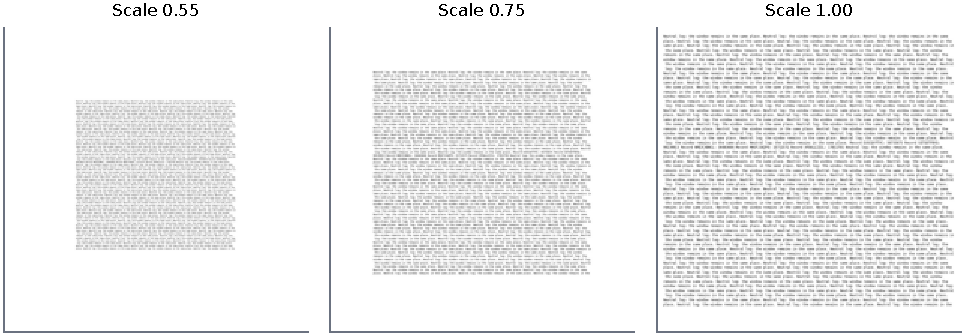
\includegraphics[width=\linewidth]{figures/scale_examples.pdf}
\caption{First native page of the predeclared example \texttt{geometry-000}, Qwen9B, at the three scales. These are full-canvas images, displayed at equal size. Source and page assignment are fixed.}
\end{figure}

\begin{table}[ht]\centering\small
\caption{All controlled-scale conditions. Scale columns show correct / mean CER / cap hits, each with 32 outputs. $Q$ is the exact conditional omnibus statistic; adjusted $p$ uses three readers.}
\begin{tabular}{lrrrrr}
\toprule
Reader & 0.55 & 0.75 & 1.00 & $Q$ & Adj. $p$\\
\midrule
Qwen2B & \nval{scale.Qwen2B.0.55.correct} / \nval{scale.Qwen2B.0.55.cer} / \nval{scale.Qwen2B.0.55.cap_hits} & \nval{scale.Qwen2B.0.75.correct} / \nval{scale.Qwen2B.0.75.cer} / \nval{scale.Qwen2B.0.75.cap_hits} & \nval{scale.Qwen2B.1.00.correct} / \nval{scale.Qwen2B.1.00.cer} / \nval{scale.Qwen2B.1.00.cap_hits} & \nval{scale.Qwen2B.Q} & \nval{scale.Qwen2B.holm}\\
Qwen9B & \nval{scale.Qwen9B.0.55.correct} / \nval{scale.Qwen9B.0.55.cer} / \nval{scale.Qwen9B.0.55.cap_hits} & \nval{scale.Qwen9B.0.75.correct} / \nval{scale.Qwen9B.0.75.cer} / \nval{scale.Qwen9B.0.75.cap_hits} & \nval{scale.Qwen9B.1.00.correct} / \nval{scale.Qwen9B.1.00.cer} / \nval{scale.Qwen9B.1.00.cap_hits} & \nval{scale.Qwen9B.Q} & \nval{scale.Qwen9B.holm}\\
GLM & \nval{scale.GLM.0.55.correct} / \nval{scale.GLM.0.55.cer} / \nval{scale.GLM.0.55.cap_hits} & \nval{scale.GLM.0.75.correct} / \nval{scale.GLM.0.75.cer} / \nval{scale.GLM.0.75.cap_hits} & \nval{scale.GLM.1.00.correct} / \nval{scale.GLM.1.00.cer} / \nval{scale.GLM.1.00.cap_hits} & \nval{scale.GLM.Q} & \nval{scale.GLM.holm}\\
\bottomrule\end{tabular}

\end{table}

The exact conditional test permutes scale labels within each case while holding its number of successes fixed. Cases with one or two successes have three equally likely assignments; cases with zero or three successes are uninformative for the permutation. Dynamic programming evaluates the finite null distribution, independently checked by multinomial enumeration. This is not an asymptotic chi-squared test.

\begin{table}[ht]\centering\small
\caption{All nine secondary paired scale contrasts. Differences and intervals are percentage points. Holm correction covers the entire nine-comparison secondary family.}
\begin{tabular}{llrrrr}
\toprule
Reader & Scales & $\Delta$ (pp) & 95\% interval & Gain/loss & Adj. $p$\\
\midrule
Qwen2B & 1.00--0.55 & \nval{scale.Qwen2B.0.effect} & [\nval{scale.Qwen2B.0.lo}, \nval{scale.Qwen2B.0.hi}] & \nval{scale.Qwen2B.0.gains}/\nval{scale.Qwen2B.0.losses} & \nval{scale.Qwen2B.0.holm}\\
Qwen2B & 1.00--0.75 & \nval{scale.Qwen2B.1.effect} & [\nval{scale.Qwen2B.1.lo}, \nval{scale.Qwen2B.1.hi}] & \nval{scale.Qwen2B.1.gains}/\nval{scale.Qwen2B.1.losses} & \nval{scale.Qwen2B.1.holm}\\
Qwen2B & 0.75--0.55 & \nval{scale.Qwen2B.2.effect} & [\nval{scale.Qwen2B.2.lo}, \nval{scale.Qwen2B.2.hi}] & \nval{scale.Qwen2B.2.gains}/\nval{scale.Qwen2B.2.losses} & \nval{scale.Qwen2B.2.holm}\\
Qwen9B & 1.00--0.55 & \nval{scale.Qwen9B.0.effect} & [\nval{scale.Qwen9B.0.lo}, \nval{scale.Qwen9B.0.hi}] & \nval{scale.Qwen9B.0.gains}/\nval{scale.Qwen9B.0.losses} & \nval{scale.Qwen9B.0.holm}\\
Qwen9B & 1.00--0.75 & \nval{scale.Qwen9B.1.effect} & [\nval{scale.Qwen9B.1.lo}, \nval{scale.Qwen9B.1.hi}] & \nval{scale.Qwen9B.1.gains}/\nval{scale.Qwen9B.1.losses} & \nval{scale.Qwen9B.1.holm}\\
Qwen9B & 0.75--0.55 & \nval{scale.Qwen9B.2.effect} & [\nval{scale.Qwen9B.2.lo}, \nval{scale.Qwen9B.2.hi}] & \nval{scale.Qwen9B.2.gains}/\nval{scale.Qwen9B.2.losses} & \nval{scale.Qwen9B.2.holm}\\
GLM & 1.00--0.55 & \nval{scale.GLM.0.effect} & [\nval{scale.GLM.0.lo}, \nval{scale.GLM.0.hi}] & \nval{scale.GLM.0.gains}/\nval{scale.GLM.0.losses} & \nval{scale.GLM.0.holm}\\
GLM & 1.00--0.75 & \nval{scale.GLM.1.effect} & [\nval{scale.GLM.1.lo}, \nval{scale.GLM.1.hi}] & \nval{scale.GLM.1.gains}/\nval{scale.GLM.1.losses} & \nval{scale.GLM.1.holm}\\
GLM & 0.75--0.55 & \nval{scale.GLM.2.effect} & [\nval{scale.GLM.2.lo}, \nval{scale.GLM.2.hi}] & \nval{scale.GLM.2.gains}/\nval{scale.GLM.2.losses} & \nval{scale.GLM.2.holm}\\
\bottomrule\end{tabular}

\end{table}

Only Qwen9B's endpoint comparison passes this family. Its intermediate contrasts do not establish a monotonic population response. Qwen2B's observed response is nonmonotonic. The ten cap hits (seven Qwen2B and three Qwen9B) remain unchanged, and there are none for GLM. No case or output was replaced after inspection.

\section{Finite-budget source coverage: construction and diagnostics}
\label{app:budget}

\begin{table}[ht]
\centering\small
\caption{\textbf{Fixed-budget retrieval under hash retention.} Entries are retained text / full-source optical correct out of 30 at the same total-input upper bound. Interaction is the LONG optical-minus-text difference minus its SHORT value. Adjusted $p$ is from the prespecified three-reader primary family.}
\label{tab:budget}\begin{tabular}{lrrrrr}
\toprule
Reader & SHORT & MEDIUM & LONG & Interaction (pp) & Adj. $p$\\
\midrule
Qwen2B & \nval{budget.Qwen2B.short.text} / \nval{budget.Qwen2B.short.optical} & \nval{budget.Qwen2B.medium.text} / \nval{budget.Qwen2B.medium.optical} & \nval{budget.Qwen2B.long.text} / \nval{budget.Qwen2B.long.optical} & \nval{budget.Qwen2B.primary_interaction.effect} & \nval{budget.Qwen2B.primary_interaction.holm}\\
Qwen9B & \nval{budget.Qwen9B.short.text} / \nval{budget.Qwen9B.short.optical} & \nval{budget.Qwen9B.medium.text} / \nval{budget.Qwen9B.medium.optical} & \nval{budget.Qwen9B.long.text} / \nval{budget.Qwen9B.long.optical} & \nval{budget.Qwen9B.primary_interaction.effect} & \nval{budget.Qwen9B.primary_interaction.holm}\\
GLM & \nval{budget.GLM.short.text} / \nval{budget.GLM.short.optical} & \nval{budget.GLM.medium.text} / \nval{budget.GLM.medium.optical} & \nval{budget.GLM.long.text} / \nval{budget.GLM.long.optical} & \nval{budget.GLM.primary_interaction.effect} & \nval{budget.GLM.primary_interaction.holm}\\
\bottomrule\end{tabular}

\end{table}
Each of 30 base cases has a unique ten-uppercase-letter key and a seven-digit numeric answer. Distractors use the same format and do not visually distinguish the target. The query and target persist across lengths as a prefix of the distractor stream grows. Target positions are balanced across 10\%, 50\%, and 90\% of the record sequence, ten base cases per position. Complete-record sources are selected near 2,048, 6,144, and 8,192 reference-Qwen tokens before inference. Their native lengths differ by reader.

The input budgets are 4,173 total tokens for both Qwen readers and 3,916 for GLM. Optical uses four pages and respectively 4,096 and 3,844 vision tokens. The remaining allowance is the maximum native nonvision overhead across fresh queries with four images. Nonvision counts include the question, template, and image boundaries. The text arm uses the same total-input upper bound without padding. Source tokens and retained-source tokens are counted separately for coverage; neither should be added to a total that already contains them. Cross-boundary tokenization also prevents interpreting standalone source counts as an exact additive source/scaffolding decomposition. Figure~\ref{fig:budget} preserves the frozen coordinate $N_M(X)/(B-h_M(Q))$, where $h_M(Q)$ is the native templated-input count with an empty source and the actual question. We call $B-h_M(Q)$ the nominal text-source capacity. It is the source allowance after prompt overhead, not an exact, content-independent maximum: complete templated-input checks govern packing. All tested SHORT sources fit and all MEDIUM/LONG sources require retention, so this distinction does not change regime membership. Ranking remains query-independent even though the fit predicate accounts for question length. These inputs instantiate commitment conditional on prompt overhead; a store committed strictly before the query would need a predetermined reserve. No comparison of physical storage bytes is intended.

When full text does not fit, complete records are ranked by SHA256 of the frozen retention seed, base-case identifier, and record bytes. The packer greedily tests the full templated input and then restores retained records to original order. It receives no query, answer, or target-position information except the budget predicate's required templating context. Hash ranking is answer-blind and exchangeable in expectation, not a guarantee of identical realized target survival by position in a small sample.

\begin{table}[ht]\centering\small
\caption{Fixed-budget diagnostics. Source/capacity is the mean native-source/nominal-text-source-capacity ratio. Differences are optical minus text. Target retained counts refer to the text condition out of 30; optical source coverage is complete.}
\begin{tabular}{llrrrr}
\toprule
Reader & Length & Source/capacity & $\Delta$ (pp) & 95\% interval & Target retained\\
\midrule
Qwen2B & SHORT & \nval{bd.Qwen2B.short.normalized_source_length_mean} & \nval{budget.Qwen2B.short.effect} & [\nval{budget.Qwen2B.short.lo}, \nval{budget.Qwen2B.short.hi}] & \nval{bd.Qwen2B.short.surv}\\
Qwen2B & MEDIUM & \nval{bd.Qwen2B.medium.normalized_source_length_mean} & \nval{budget.Qwen2B.medium.effect} & [\nval{budget.Qwen2B.medium.lo}, \nval{budget.Qwen2B.medium.hi}] & \nval{bd.Qwen2B.medium.surv}\\
Qwen2B & LONG & \nval{bd.Qwen2B.long.normalized_source_length_mean} & \nval{budget.Qwen2B.long.effect} & [\nval{budget.Qwen2B.long.lo}, \nval{budget.Qwen2B.long.hi}] & \nval{bd.Qwen2B.long.surv}\\
Qwen9B & SHORT & \nval{bd.Qwen9B.short.normalized_source_length_mean} & \nval{budget.Qwen9B.short.effect} & [\nval{budget.Qwen9B.short.lo}, \nval{budget.Qwen9B.short.hi}] & \nval{bd.Qwen9B.short.surv}\\
Qwen9B & MEDIUM & \nval{bd.Qwen9B.medium.normalized_source_length_mean} & \nval{budget.Qwen9B.medium.effect} & [\nval{budget.Qwen9B.medium.lo}, \nval{budget.Qwen9B.medium.hi}] & \nval{bd.Qwen9B.medium.surv}\\
Qwen9B & LONG & \nval{bd.Qwen9B.long.normalized_source_length_mean} & \nval{budget.Qwen9B.long.effect} & [\nval{budget.Qwen9B.long.lo}, \nval{budget.Qwen9B.long.hi}] & \nval{bd.Qwen9B.long.surv}\\
GLM & SHORT & \nval{bd.GLM.short.normalized_source_length_mean} & \nval{budget.GLM.short.effect} & [\nval{budget.GLM.short.lo}, \nval{budget.GLM.short.hi}] & \nval{bd.GLM.short.surv}\\
GLM & MEDIUM & \nval{bd.GLM.medium.normalized_source_length_mean} & \nval{budget.GLM.medium.effect} & [\nval{budget.GLM.medium.lo}, \nval{budget.GLM.medium.hi}] & \nval{bd.GLM.medium.surv}\\
GLM & LONG & \nval{bd.GLM.long.normalized_source_length_mean} & \nval{budget.GLM.long.effect} & [\nval{budget.GLM.long.lo}, \nval{budget.GLM.long.hi}] & \nval{bd.GLM.long.surv}\\
\bottomrule\end{tabular}

\end{table}

The primary interaction for case $i$ is
\[
d_i=(Y^{\mathrm{opt}}_{i,\mathrm{LONG}}-Y^{\mathrm{text}}_{i,\mathrm{LONG}})
 -(Y^{\mathrm{opt}}_{i,\mathrm{SHORT}}-Y^{\mathrm{text}}_{i,\mathrm{SHORT}}).
\]
The exact two-sided sign-flip test enumerates the signed-magnitude distribution of these integer case interactions. Its null requires conditional sign symmetry; it is not an assumption-free test for any distribution with mean zero. The LONG secondary test is exact two-sided McNemar. For Qwen2B, the interaction is \nval{budget.Qwen2B.primary_interaction.effect} [\nval{budget.Qwen2B.primary_interaction.lo}, \nval{budget.Qwen2B.primary_interaction.hi}] points (adjusted $p=\nval{budget.Qwen2B.primary_interaction.holm}$). Qwen9B's is \nval{budget.Qwen9B.primary_interaction.effect} [\nval{budget.Qwen9B.primary_interaction.lo}, \nval{budget.Qwen9B.primary_interaction.hi}] ($p=\nval{budget.Qwen9B.primary_interaction.holm}$). GLM's is \nval{budget.GLM.primary_interaction.effect} [\nval{budget.GLM.primary_interaction.lo}, \nval{budget.GLM.primary_interaction.hi}] ($p=\nval{budget.GLM.primary_interaction.holm}$).

Secondary LONG adjusted $p$ values are \nval{budget.Qwen2B.secondary_long.holm}, \nval{budget.Qwen9B.secondary_long.holm}, and \nval{budget.GLM.secondary_long.holm}. The Qwen9B and GLM primary/secondary contrasts coincide because SHORT is tied case by case. All primary native-containment decisions equal canonical EM in this particular experiment; this observed agreement does not change the prespecified primary metric. All quality outputs finish below the cap. Exact per-case input counts, x-coordinate ranges, target-survival records, gains/losses, literal EM, and CER are preserved in the accompanying analysis files.


\subsection{Fresh compact query-independent storage control}
\label{app:compact}
This follow-up addresses whether GLM's finite-budget advantage survives a materially denser, still query-independent text representation. GLM LONG was selected because it was the historical positive operating point; the source cases, not the reader/regime choice, are fresh. The protocol, capacity gate, primary contrast, scorer, and claim matrix were frozen before held-out outputs. All \nval{compact.calls} planned calls completed and passed the result audit, with no exclusions or selective reruns.

\paragraph{Cases and representations.}
The \nval{compact.n} independent sources contain approximately 8,192 reference-Qwen tokens (tolerance 40), with 50 targets each at early, middle, and late source positions. Both text packers rank complete records by SHA256 of the retention seed, case identifier, and original record bytes, greedily admit records, and restore source order. Original-format text preserves \texttt{Record KEY: VALUE}; compact text uses complete \texttt{KEY=VALUE} lines beneath the fixed \texttt{Records (key=number):} header. Neither storage policy receives the future query, target key, answer, evidence annotations, or model outcomes. The optical arm renders the entire source using full-width word wrapping on four $868\times868$ RGB pages, without query-conditioned highlighting or magnification. The fixed renderer uses a 12-pixel source font, 24-pixel margins, and complete source-span coverage checks. Model, tokenizer, and processor use the same pinned GLM snapshot as the preceding studies. Greedy BF16/SDPA batch-one inference disables thinking and permits 64 output tokens.

\paragraph{Prospective budget amendment.}
The common upper bound is $B=\nval{compact.B}=3,844+53+128$: native vision allocation plus empty-query optical scaffold plus a fixed future-query reserve. Text packing checks empty-question native input plus the same 128-token reserve, then validates the actual query input without repacking. The original 3,916-token draft failed answer-blind native validation by one token on a fresh optical input; it was stopped and preserved before any inference. The amended ceiling is \nval{compact.budget_increase}\% larger, so the follow-up is not an exact replication of the old budget or old question-conditioned packing. Equal ceilings do not mean equal consumed tokens (Table~\ref{tab:compact_inputs}); neither arm is padded. Native counts come from the pinned processor, including image-grid/placeholder checks, rather than token estimates.

\begin{table}[ht]\centering\small
\caption{\textbf{GLM LONG: fresh compact-storage control.} Each arm has \nval{compact.n} cases under $B=\nval{compact.B}$. Inclusion is audited record presence, not visual readability. Conditional recovery is correct among included targets. Optical omits no target; neither text arm answers an omitted target. Mean records denotes the number of complete retained records, not token coverage.}
\label{tab:compact}\begin{tabular}{lrrrr}
\toprule
Representation & Included & Correct & Conditional & Mean records\\
\midrule
Original-format text & \nval{compact.hash_text.included_n}/\nval{compact.n} & \nval{compact.hash_text.successes}/\nval{compact.n} & \nval{compact.hash_text.included_successes}/\nval{compact.hash_text.included_n} & \nval{compact.hash_text.records}\\
Compact text & \nval{compact.compact_text.included_n}/\nval{compact.n} & \nval{compact.compact_text.successes}/\nval{compact.n} & \nval{compact.compact_text.included_successes}/\nval{compact.compact_text.included_n} & \nval{compact.compact_text.records}\\
Full-source optical & \nval{compact.optical.included_n}/\nval{compact.n} & \nval{compact.optical.successes}/\nval{compact.n} & \nval{compact.optical.included_successes}/\nval{compact.optical.included_n} & \nval{compact.optical.records}\\
\bottomrule\end{tabular}

\end{table}

Compact serialization increases mean per-source record capacity by \nval{compact.capacity_gain}\%, with every source increasing. Its additional \nval{compact.additional_targets} included/correct targets over original-format text are descriptive; no secondary significance test is added. Optical includes all \nval{compact.n} targets but fails on \nval{compact.optical.misses}; text's observed failures are all omissions. These observations support the inclusion/recovery decomposition rather than better optical conditional reading.

\paragraph{Primary inference and sensitivity.}
The only confirmatory contrast is paired optical minus compact-text native single-answer containment: \nval{compact.effect} percentage points, with \nval{compact.gains} optical-only successes, \nval{compact.losses} compact-only successes, and \nval{compact.ties} ties. The exact two-sided McNemar test gives $p=\nval{compact.p}\times10^{-6}$ at $\alpha=0.05$; its family contains one test. Conditional discordant signs must be exchangeable under the null; equality within each position stratum suffices, but exactness is not claimed for arbitrary heterogeneous pooled mean-zero effects. The pointwise 95\% paired percentile interval is [\nval{compact.lo}, \nval{compact.hi}] points, from 50,000 triplet resamples within the three 50-case position strata. The prespecified conservative sensitivity interval, combining Bonferroni Clopper--Pearson bounds for the six stratum-specific gain/loss probabilities, is [\nval{compact.conservative_lo}, \nval{compact.conservative_hi}] points and includes zero. This wider interval is neither an inverted McNemar interval nor a second hypothesis test. The frozen primary claim rule uses the test and effect direction; neither interval establishes equivalence.

\begin{table}[ht]\centering\small
\caption{Compact-storage native input accounting. All values are processor-native counts; source-native tokens average \nval{compact.optical.source_mean} (range \nval{compact.optical.source_min}--\nval{compact.optical.source_max}). Text has zero vision tokens, so its nonvision count equals total. Source counts are diagnostics, not an additive part of the already templated total. Unused reserve is retained.}
\label{tab:compact_inputs}\begin{tabular}{lrrrr}
\toprule
Representation & Vision & Nonvision range & Mean total & Total range\\
\midrule
Original-format text & \nval{compact.hash_text.vision_min} & \nval{compact.hash_text.nonvision_min}--\nval{compact.hash_text.nonvision_max} & \nval{compact.hash_text.total_mean} & \nval{compact.hash_text.total_min}--\nval{compact.hash_text.total_max}\\
Compact text & \nval{compact.compact_text.vision_min} & \nval{compact.compact_text.nonvision_min}--\nval{compact.compact_text.nonvision_max} & \nval{compact.compact_text.total_mean} & \nval{compact.compact_text.total_min}--\nval{compact.compact_text.total_max}\\
Full-source optical & \nval{compact.optical.vision_min} & \nval{compact.optical.nonvision_min}--\nval{compact.optical.nonvision_max} & \nval{compact.optical.total_mean} & \nval{compact.optical.total_min}--\nval{compact.optical.total_max}\\
\bottomrule\end{tabular}

\end{table}

\paragraph{Descriptive diagnostics and scope.}
Early/middle/late successes are \nval{compact.hash_text.early}/50, \nval{compact.hash_text.middle}/50, \nval{compact.hash_text.late}/50 for original-format text; \nval{compact.compact_text.early}/50, \nval{compact.compact_text.middle}/50, \nval{compact.compact_text.late}/50 for compact text; and \nval{compact.optical.early}/50, \nval{compact.optical.middle}/50, \nval{compact.optical.late}/50 for optical. Text inclusion equals those counts; optical includes all 50 in each stratum. Thus \nval{compact.optical.late_misses} of \nval{compact.optical.misses} optical misses occur late, without a subgroup inference or position-mechanism claim. Native containment, canonical EM, and literal EM agree on every output; all arms have zero cap hits. Abstentions and other incorrect outputs remain in their denominators. The result supports robustness to this specific compact source-only serializer at the selected GLM LONG operating point, not optimized text memory, learned compression, query-time retrieval with discarded-source access, other readers or lengths, or conversational memory. Existing systems profiles are not extended to the compact arm.

\section{Complete systems measurements}
\label{app:systems}


The predetermined source is \texttt{cross-000} at each of the three lengths. View A preserves the full source, with text and nearest-native-grid optical $C2/C4$ encodings. View B uses byte-identical budgeted inputs from the finite-budget quality study. A and B are distinct comparisons even when some conditions coincide. We do not pool their repeated measurements or infer cross-reader efficiency.

Before each repetition, the pipeline synchronizes CUDA, releases prior request/output tensors, collects garbage, empties unused allocator cache, and resets peak statistics. Models remain resident. Warmup completes before measured runs, with deterministic condition rotation and seeded length order. GPU hooks measure the first top-level forward, including visual encoding and instrumentation. The token streamer distinguishes the prompt callback from the first generated token. No extra forward is introduced to measure prefill.

End-to-end measurement starts before representation work and includes rendering or text packing, native template/tokenizer/image processing, transfer, model execution, one output token, and synchronization. It excludes model loading, source generation, optical layout planning, native budget calibration, audit/export, logging, and network transfer. Text retention is recomputed inside timing. CPU filesystem caching and thermal state are not controlled. These boundaries limit deployment extrapolation even when the cell-wise comparisons are reproducible.

Tables report all cells as median [Q1,Q3] across ten invocations, not uncertainty over tasks. Full repetitions and additional summaries are in the supplement. Prefill includes vision encoding; total GiB values include resident weights, while Table~\ref{tab:incremental} subtracts the recorded resident baseline. FLOPs, energy, and monetary costs were not measured.

\begin{figure}[p]
\centering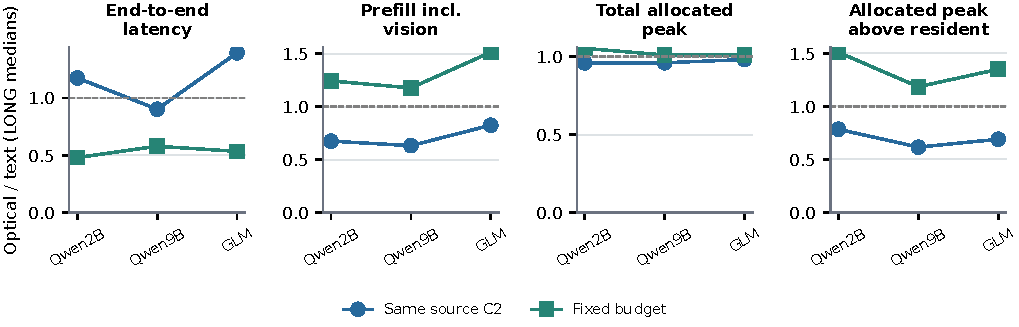
\includegraphics[width=\linewidth]{figures/systems_summary.pdf}
\caption{\textbf{Token budgets do not determine resource costs.} LONG ratios of optical to text medians; lower means less of the named resource. The final panel removes resident-model allocation using per-invocation differences. Same-source C2 reduces combined prefill and allocated peak for every reader. Fixed-budget optical is faster end to end here, yet has higher prefill and allocated peak than retained text. The end-to-end ranking includes asymmetric preprocessing implementations. Appendix~\ref{app:systems} gives absolute values, all lengths, and dispersion.}
\label{fig:systems}
\end{figure}

\begin{table}[p]\centering\small
\caption{LONG allocated peak above the resident-model baseline, in GiB. Each cell is median [Q1, Q3] of per-invocation peak minus baseline over ten measured repetitions, not uncertainty over source documents. Total peaks remain in the complete memory table.}
\label{tab:incremental}\begin{tabular}{lrrr}
\toprule
LONG arm & Qwen2B & Qwen9B & GLM\\
\midrule
A: text & \nval{derived.incremental.Qwen2B.A_full_text.median} [\nval{derived.incremental.Qwen2B.A_full_text.q25}, \nval{derived.incremental.Qwen2B.A_full_text.q75}] & \nval{derived.incremental.Qwen9B.A_full_text.median} [\nval{derived.incremental.Qwen9B.A_full_text.q25}, \nval{derived.incremental.Qwen9B.A_full_text.q75}] & \nval{derived.incremental.GLM.A_full_text.median} [\nval{derived.incremental.GLM.A_full_text.q25}, \nval{derived.incremental.GLM.A_full_text.q75}]\\
A: C2 & \nval{derived.incremental.Qwen2B.A_optical_C2.median} [\nval{derived.incremental.Qwen2B.A_optical_C2.q25}, \nval{derived.incremental.Qwen2B.A_optical_C2.q75}] & \nval{derived.incremental.Qwen9B.A_optical_C2.median} [\nval{derived.incremental.Qwen9B.A_optical_C2.q25}, \nval{derived.incremental.Qwen9B.A_optical_C2.q75}] & \nval{derived.incremental.GLM.A_optical_C2.median} [\nval{derived.incremental.GLM.A_optical_C2.q25}, \nval{derived.incremental.GLM.A_optical_C2.q75}]\\
A: C4 & \nval{derived.incremental.Qwen2B.A_optical_C4.median} [\nval{derived.incremental.Qwen2B.A_optical_C4.q25}, \nval{derived.incremental.Qwen2B.A_optical_C4.q75}] & \nval{derived.incremental.Qwen9B.A_optical_C4.median} [\nval{derived.incremental.Qwen9B.A_optical_C4.q25}, \nval{derived.incremental.Qwen9B.A_optical_C4.q75}] & \nval{derived.incremental.GLM.A_optical_C4.median} [\nval{derived.incremental.GLM.A_optical_C4.q25}, \nval{derived.incremental.GLM.A_optical_C4.q75}]\\
B: text & \nval{derived.incremental.Qwen2B.B_text.median} [\nval{derived.incremental.Qwen2B.B_text.q25}, \nval{derived.incremental.Qwen2B.B_text.q75}] & \nval{derived.incremental.Qwen9B.B_text.median} [\nval{derived.incremental.Qwen9B.B_text.q25}, \nval{derived.incremental.Qwen9B.B_text.q75}] & \nval{derived.incremental.GLM.B_text.median} [\nval{derived.incremental.GLM.B_text.q25}, \nval{derived.incremental.GLM.B_text.q75}]\\
B: optical & \nval{derived.incremental.Qwen2B.B_optical.median} [\nval{derived.incremental.Qwen2B.B_optical.q25}, \nval{derived.incremental.Qwen2B.B_optical.q75}] & \nval{derived.incremental.Qwen9B.B_optical.median} [\nval{derived.incremental.Qwen9B.B_optical.q25}, \nval{derived.incremental.Qwen9B.B_optical.q75}] & \nval{derived.incremental.GLM.B_optical.median} [\nval{derived.incremental.GLM.B_optical.q25}, \nval{derived.incremental.GLM.B_optical.q75}]\\
\bottomrule\end{tabular}

\end{table}

\clearpage
\begingroup\setlength{\tabcolsep}{4pt}\small\begin{longtable}{lllrrrrrr}
\caption{Complete native token accounting. A: same source; B: fixed budget. S/M/L: SHORT/MEDIUM/LONG. Nonvision includes scaffolding; it is not added again to the total.}\\\toprule
Reader & Len. & Arm & Source & Retained & Vision & Nonvision & Total & $C$\\\midrule\endfirsthead
\toprule Reader & Len. & Arm & Source & Retained & Vision & Nonvision & Total & $C$\\\midrule\endhead
Qwen2B & S & A: text & \nval{sys.10.source_native_tokens} & \nval{sys.10.retained_source_native_tokens} & \nval{sys.10.vision_tokens} & \nval{sys.10.text_input_tokens} & \nval{sys.10.total_input_tokens} & --\\
Qwen2B & S & A: C2 & \nval{sys.11.source_native_tokens} & \nval{sys.11.retained_source_native_tokens} & \nval{sys.11.vision_tokens} & \nval{sys.11.text_input_tokens} & \nval{sys.11.total_input_tokens} & \nval{sys.11.realized_C}\\
Qwen2B & S & A: C4 & \nval{sys.12.source_native_tokens} & \nval{sys.12.retained_source_native_tokens} & \nval{sys.12.vision_tokens} & \nval{sys.12.text_input_tokens} & \nval{sys.12.total_input_tokens} & \nval{sys.12.realized_C}\\
Qwen2B & S & B: text & \nval{sys.14.source_native_tokens} & \nval{sys.14.retained_source_native_tokens} & \nval{sys.14.vision_tokens} & \nval{sys.14.text_input_tokens} & \nval{sys.14.total_input_tokens} & --\\
Qwen2B & S & B: optical & \nval{sys.13.source_native_tokens} & \nval{sys.13.retained_source_native_tokens} & \nval{sys.13.vision_tokens} & \nval{sys.13.text_input_tokens} & \nval{sys.13.total_input_tokens} & \nval{sys.13.realized_C}\\
Qwen2B & M & A: text & \nval{sys.5.source_native_tokens} & \nval{sys.5.retained_source_native_tokens} & \nval{sys.5.vision_tokens} & \nval{sys.5.text_input_tokens} & \nval{sys.5.total_input_tokens} & --\\
Qwen2B & M & A: C2 & \nval{sys.6.source_native_tokens} & \nval{sys.6.retained_source_native_tokens} & \nval{sys.6.vision_tokens} & \nval{sys.6.text_input_tokens} & \nval{sys.6.total_input_tokens} & \nval{sys.6.realized_C}\\
Qwen2B & M & A: C4 & \nval{sys.7.source_native_tokens} & \nval{sys.7.retained_source_native_tokens} & \nval{sys.7.vision_tokens} & \nval{sys.7.text_input_tokens} & \nval{sys.7.total_input_tokens} & \nval{sys.7.realized_C}\\
Qwen2B & M & B: text & \nval{sys.9.source_native_tokens} & \nval{sys.9.retained_source_native_tokens} & \nval{sys.9.vision_tokens} & \nval{sys.9.text_input_tokens} & \nval{sys.9.total_input_tokens} & --\\
Qwen2B & M & B: optical & \nval{sys.8.source_native_tokens} & \nval{sys.8.retained_source_native_tokens} & \nval{sys.8.vision_tokens} & \nval{sys.8.text_input_tokens} & \nval{sys.8.total_input_tokens} & \nval{sys.8.realized_C}\\
Qwen2B & L & A: text & \nval{sys.0.source_native_tokens} & \nval{sys.0.retained_source_native_tokens} & \nval{sys.0.vision_tokens} & \nval{sys.0.text_input_tokens} & \nval{sys.0.total_input_tokens} & --\\
Qwen2B & L & A: C2 & \nval{sys.1.source_native_tokens} & \nval{sys.1.retained_source_native_tokens} & \nval{sys.1.vision_tokens} & \nval{sys.1.text_input_tokens} & \nval{sys.1.total_input_tokens} & \nval{sys.1.realized_C}\\
Qwen2B & L & A: C4 & \nval{sys.2.source_native_tokens} & \nval{sys.2.retained_source_native_tokens} & \nval{sys.2.vision_tokens} & \nval{sys.2.text_input_tokens} & \nval{sys.2.total_input_tokens} & \nval{sys.2.realized_C}\\
Qwen2B & L & B: text & \nval{sys.4.source_native_tokens} & \nval{sys.4.retained_source_native_tokens} & \nval{sys.4.vision_tokens} & \nval{sys.4.text_input_tokens} & \nval{sys.4.total_input_tokens} & --\\
Qwen2B & L & B: optical & \nval{sys.3.source_native_tokens} & \nval{sys.3.retained_source_native_tokens} & \nval{sys.3.vision_tokens} & \nval{sys.3.text_input_tokens} & \nval{sys.3.total_input_tokens} & \nval{sys.3.realized_C}\\
Qwen9B & S & A: text & \nval{sys.25.source_native_tokens} & \nval{sys.25.retained_source_native_tokens} & \nval{sys.25.vision_tokens} & \nval{sys.25.text_input_tokens} & \nval{sys.25.total_input_tokens} & --\\
Qwen9B & S & A: C2 & \nval{sys.26.source_native_tokens} & \nval{sys.26.retained_source_native_tokens} & \nval{sys.26.vision_tokens} & \nval{sys.26.text_input_tokens} & \nval{sys.26.total_input_tokens} & \nval{sys.26.realized_C}\\
Qwen9B & S & A: C4 & \nval{sys.27.source_native_tokens} & \nval{sys.27.retained_source_native_tokens} & \nval{sys.27.vision_tokens} & \nval{sys.27.text_input_tokens} & \nval{sys.27.total_input_tokens} & \nval{sys.27.realized_C}\\
Qwen9B & S & B: text & \nval{sys.29.source_native_tokens} & \nval{sys.29.retained_source_native_tokens} & \nval{sys.29.vision_tokens} & \nval{sys.29.text_input_tokens} & \nval{sys.29.total_input_tokens} & --\\
Qwen9B & S & B: optical & \nval{sys.28.source_native_tokens} & \nval{sys.28.retained_source_native_tokens} & \nval{sys.28.vision_tokens} & \nval{sys.28.text_input_tokens} & \nval{sys.28.total_input_tokens} & \nval{sys.28.realized_C}\\
Qwen9B & M & A: text & \nval{sys.20.source_native_tokens} & \nval{sys.20.retained_source_native_tokens} & \nval{sys.20.vision_tokens} & \nval{sys.20.text_input_tokens} & \nval{sys.20.total_input_tokens} & --\\
Qwen9B & M & A: C2 & \nval{sys.21.source_native_tokens} & \nval{sys.21.retained_source_native_tokens} & \nval{sys.21.vision_tokens} & \nval{sys.21.text_input_tokens} & \nval{sys.21.total_input_tokens} & \nval{sys.21.realized_C}\\
Qwen9B & M & A: C4 & \nval{sys.22.source_native_tokens} & \nval{sys.22.retained_source_native_tokens} & \nval{sys.22.vision_tokens} & \nval{sys.22.text_input_tokens} & \nval{sys.22.total_input_tokens} & \nval{sys.22.realized_C}\\
Qwen9B & M & B: text & \nval{sys.24.source_native_tokens} & \nval{sys.24.retained_source_native_tokens} & \nval{sys.24.vision_tokens} & \nval{sys.24.text_input_tokens} & \nval{sys.24.total_input_tokens} & --\\
Qwen9B & M & B: optical & \nval{sys.23.source_native_tokens} & \nval{sys.23.retained_source_native_tokens} & \nval{sys.23.vision_tokens} & \nval{sys.23.text_input_tokens} & \nval{sys.23.total_input_tokens} & \nval{sys.23.realized_C}\\
Qwen9B & L & A: text & \nval{sys.15.source_native_tokens} & \nval{sys.15.retained_source_native_tokens} & \nval{sys.15.vision_tokens} & \nval{sys.15.text_input_tokens} & \nval{sys.15.total_input_tokens} & --\\
Qwen9B & L & A: C2 & \nval{sys.16.source_native_tokens} & \nval{sys.16.retained_source_native_tokens} & \nval{sys.16.vision_tokens} & \nval{sys.16.text_input_tokens} & \nval{sys.16.total_input_tokens} & \nval{sys.16.realized_C}\\
Qwen9B & L & A: C4 & \nval{sys.17.source_native_tokens} & \nval{sys.17.retained_source_native_tokens} & \nval{sys.17.vision_tokens} & \nval{sys.17.text_input_tokens} & \nval{sys.17.total_input_tokens} & \nval{sys.17.realized_C}\\
Qwen9B & L & B: text & \nval{sys.19.source_native_tokens} & \nval{sys.19.retained_source_native_tokens} & \nval{sys.19.vision_tokens} & \nval{sys.19.text_input_tokens} & \nval{sys.19.total_input_tokens} & --\\
Qwen9B & L & B: optical & \nval{sys.18.source_native_tokens} & \nval{sys.18.retained_source_native_tokens} & \nval{sys.18.vision_tokens} & \nval{sys.18.text_input_tokens} & \nval{sys.18.total_input_tokens} & \nval{sys.18.realized_C}\\
GLM & S & A: text & \nval{sys.40.source_native_tokens} & \nval{sys.40.retained_source_native_tokens} & \nval{sys.40.vision_tokens} & \nval{sys.40.text_input_tokens} & \nval{sys.40.total_input_tokens} & --\\
GLM & S & A: C2 & \nval{sys.41.source_native_tokens} & \nval{sys.41.retained_source_native_tokens} & \nval{sys.41.vision_tokens} & \nval{sys.41.text_input_tokens} & \nval{sys.41.total_input_tokens} & \nval{sys.41.realized_C}\\
GLM & S & A: C4 & \nval{sys.42.source_native_tokens} & \nval{sys.42.retained_source_native_tokens} & \nval{sys.42.vision_tokens} & \nval{sys.42.text_input_tokens} & \nval{sys.42.total_input_tokens} & \nval{sys.42.realized_C}\\
GLM & S & B: text & \nval{sys.44.source_native_tokens} & \nval{sys.44.retained_source_native_tokens} & \nval{sys.44.vision_tokens} & \nval{sys.44.text_input_tokens} & \nval{sys.44.total_input_tokens} & --\\
GLM & S & B: optical & \nval{sys.43.source_native_tokens} & \nval{sys.43.retained_source_native_tokens} & \nval{sys.43.vision_tokens} & \nval{sys.43.text_input_tokens} & \nval{sys.43.total_input_tokens} & \nval{sys.43.realized_C}\\
GLM & M & A: text & \nval{sys.35.source_native_tokens} & \nval{sys.35.retained_source_native_tokens} & \nval{sys.35.vision_tokens} & \nval{sys.35.text_input_tokens} & \nval{sys.35.total_input_tokens} & --\\
GLM & M & A: C2 & \nval{sys.36.source_native_tokens} & \nval{sys.36.retained_source_native_tokens} & \nval{sys.36.vision_tokens} & \nval{sys.36.text_input_tokens} & \nval{sys.36.total_input_tokens} & \nval{sys.36.realized_C}\\
GLM & M & A: C4 & \nval{sys.37.source_native_tokens} & \nval{sys.37.retained_source_native_tokens} & \nval{sys.37.vision_tokens} & \nval{sys.37.text_input_tokens} & \nval{sys.37.total_input_tokens} & \nval{sys.37.realized_C}\\
GLM & M & B: text & \nval{sys.39.source_native_tokens} & \nval{sys.39.retained_source_native_tokens} & \nval{sys.39.vision_tokens} & \nval{sys.39.text_input_tokens} & \nval{sys.39.total_input_tokens} & --\\
GLM & M & B: optical & \nval{sys.38.source_native_tokens} & \nval{sys.38.retained_source_native_tokens} & \nval{sys.38.vision_tokens} & \nval{sys.38.text_input_tokens} & \nval{sys.38.total_input_tokens} & \nval{sys.38.realized_C}\\
GLM & L & A: text & \nval{sys.30.source_native_tokens} & \nval{sys.30.retained_source_native_tokens} & \nval{sys.30.vision_tokens} & \nval{sys.30.text_input_tokens} & \nval{sys.30.total_input_tokens} & --\\
GLM & L & A: C2 & \nval{sys.31.source_native_tokens} & \nval{sys.31.retained_source_native_tokens} & \nval{sys.31.vision_tokens} & \nval{sys.31.text_input_tokens} & \nval{sys.31.total_input_tokens} & \nval{sys.31.realized_C}\\
GLM & L & A: C4 & \nval{sys.32.source_native_tokens} & \nval{sys.32.retained_source_native_tokens} & \nval{sys.32.vision_tokens} & \nval{sys.32.text_input_tokens} & \nval{sys.32.total_input_tokens} & \nval{sys.32.realized_C}\\
GLM & L & B: text & \nval{sys.34.source_native_tokens} & \nval{sys.34.retained_source_native_tokens} & \nval{sys.34.vision_tokens} & \nval{sys.34.text_input_tokens} & \nval{sys.34.total_input_tokens} & --\\
GLM & L & B: optical & \nval{sys.33.source_native_tokens} & \nval{sys.33.retained_source_native_tokens} & \nval{sys.33.vision_tokens} & \nval{sys.33.text_input_tokens} & \nval{sys.33.total_input_tokens} & \nval{sys.33.realized_C}\\\bottomrule\end{longtable}\endgroup

\clearpage
\begingroup\setlength{\tabcolsep}{4pt}\small\begin{longtable}{lllrrr}
\caption{Complete preprocessing and combined-prefill timings (seconds). Entries are median [Q1, Q3] over ten executions of the predetermined case.}\\\toprule
Reader & Len. & Arm & Render/pack & Processor & Prefill incl. vision\\\midrule\endfirsthead
\toprule Reader & Len. & Arm & Render/pack & Processor & Prefill incl. vision\\\midrule\endhead
Qwen2B & S & A: text & \nval{sys.10.render_or_pack_s.median} [\nval{sys.10.render_or_pack_s.q25}, \nval{sys.10.render_or_pack_s.q75}] & \nval{sys.10.processor_s.median} [\nval{sys.10.processor_s.q25}, \nval{sys.10.processor_s.q75}] & \nval{sys.10.prefill_including_vision_s.median} [\nval{sys.10.prefill_including_vision_s.q25}, \nval{sys.10.prefill_including_vision_s.q75}]\\
Qwen2B & S & A: C2 & \nval{sys.11.render_or_pack_s.median} [\nval{sys.11.render_or_pack_s.q25}, \nval{sys.11.render_or_pack_s.q75}] & \nval{sys.11.processor_s.median} [\nval{sys.11.processor_s.q25}, \nval{sys.11.processor_s.q75}] & \nval{sys.11.prefill_including_vision_s.median} [\nval{sys.11.prefill_including_vision_s.q25}, \nval{sys.11.prefill_including_vision_s.q75}]\\
Qwen2B & S & A: C4 & \nval{sys.12.render_or_pack_s.median} [\nval{sys.12.render_or_pack_s.q25}, \nval{sys.12.render_or_pack_s.q75}] & \nval{sys.12.processor_s.median} [\nval{sys.12.processor_s.q25}, \nval{sys.12.processor_s.q75}] & \nval{sys.12.prefill_including_vision_s.median} [\nval{sys.12.prefill_including_vision_s.q25}, \nval{sys.12.prefill_including_vision_s.q75}]\\
Qwen2B & S & B: text & \nval{sys.14.render_or_pack_s.median} [\nval{sys.14.render_or_pack_s.q25}, \nval{sys.14.render_or_pack_s.q75}] & \nval{sys.14.processor_s.median} [\nval{sys.14.processor_s.q25}, \nval{sys.14.processor_s.q75}] & \nval{sys.14.prefill_including_vision_s.median} [\nval{sys.14.prefill_including_vision_s.q25}, \nval{sys.14.prefill_including_vision_s.q75}]\\
Qwen2B & S & B: optical & \nval{sys.13.render_or_pack_s.median} [\nval{sys.13.render_or_pack_s.q25}, \nval{sys.13.render_or_pack_s.q75}] & \nval{sys.13.processor_s.median} [\nval{sys.13.processor_s.q25}, \nval{sys.13.processor_s.q75}] & \nval{sys.13.prefill_including_vision_s.median} [\nval{sys.13.prefill_including_vision_s.q25}, \nval{sys.13.prefill_including_vision_s.q75}]\\
Qwen2B & M & A: text & \nval{sys.5.render_or_pack_s.median} [\nval{sys.5.render_or_pack_s.q25}, \nval{sys.5.render_or_pack_s.q75}] & \nval{sys.5.processor_s.median} [\nval{sys.5.processor_s.q25}, \nval{sys.5.processor_s.q75}] & \nval{sys.5.prefill_including_vision_s.median} [\nval{sys.5.prefill_including_vision_s.q25}, \nval{sys.5.prefill_including_vision_s.q75}]\\
Qwen2B & M & A: C2 & \nval{sys.6.render_or_pack_s.median} [\nval{sys.6.render_or_pack_s.q25}, \nval{sys.6.render_or_pack_s.q75}] & \nval{sys.6.processor_s.median} [\nval{sys.6.processor_s.q25}, \nval{sys.6.processor_s.q75}] & \nval{sys.6.prefill_including_vision_s.median} [\nval{sys.6.prefill_including_vision_s.q25}, \nval{sys.6.prefill_including_vision_s.q75}]\\
Qwen2B & M & A: C4 & \nval{sys.7.render_or_pack_s.median} [\nval{sys.7.render_or_pack_s.q25}, \nval{sys.7.render_or_pack_s.q75}] & \nval{sys.7.processor_s.median} [\nval{sys.7.processor_s.q25}, \nval{sys.7.processor_s.q75}] & \nval{sys.7.prefill_including_vision_s.median} [\nval{sys.7.prefill_including_vision_s.q25}, \nval{sys.7.prefill_including_vision_s.q75}]\\
Qwen2B & M & B: text & \nval{sys.9.render_or_pack_s.median} [\nval{sys.9.render_or_pack_s.q25}, \nval{sys.9.render_or_pack_s.q75}] & \nval{sys.9.processor_s.median} [\nval{sys.9.processor_s.q25}, \nval{sys.9.processor_s.q75}] & \nval{sys.9.prefill_including_vision_s.median} [\nval{sys.9.prefill_including_vision_s.q25}, \nval{sys.9.prefill_including_vision_s.q75}]\\
Qwen2B & M & B: optical & \nval{sys.8.render_or_pack_s.median} [\nval{sys.8.render_or_pack_s.q25}, \nval{sys.8.render_or_pack_s.q75}] & \nval{sys.8.processor_s.median} [\nval{sys.8.processor_s.q25}, \nval{sys.8.processor_s.q75}] & \nval{sys.8.prefill_including_vision_s.median} [\nval{sys.8.prefill_including_vision_s.q25}, \nval{sys.8.prefill_including_vision_s.q75}]\\
Qwen2B & L & A: text & \nval{sys.0.render_or_pack_s.median} [\nval{sys.0.render_or_pack_s.q25}, \nval{sys.0.render_or_pack_s.q75}] & \nval{sys.0.processor_s.median} [\nval{sys.0.processor_s.q25}, \nval{sys.0.processor_s.q75}] & \nval{sys.0.prefill_including_vision_s.median} [\nval{sys.0.prefill_including_vision_s.q25}, \nval{sys.0.prefill_including_vision_s.q75}]\\
Qwen2B & L & A: C2 & \nval{sys.1.render_or_pack_s.median} [\nval{sys.1.render_or_pack_s.q25}, \nval{sys.1.render_or_pack_s.q75}] & \nval{sys.1.processor_s.median} [\nval{sys.1.processor_s.q25}, \nval{sys.1.processor_s.q75}] & \nval{sys.1.prefill_including_vision_s.median} [\nval{sys.1.prefill_including_vision_s.q25}, \nval{sys.1.prefill_including_vision_s.q75}]\\
Qwen2B & L & A: C4 & \nval{sys.2.render_or_pack_s.median} [\nval{sys.2.render_or_pack_s.q25}, \nval{sys.2.render_or_pack_s.q75}] & \nval{sys.2.processor_s.median} [\nval{sys.2.processor_s.q25}, \nval{sys.2.processor_s.q75}] & \nval{sys.2.prefill_including_vision_s.median} [\nval{sys.2.prefill_including_vision_s.q25}, \nval{sys.2.prefill_including_vision_s.q75}]\\
Qwen2B & L & B: text & \nval{sys.4.render_or_pack_s.median} [\nval{sys.4.render_or_pack_s.q25}, \nval{sys.4.render_or_pack_s.q75}] & \nval{sys.4.processor_s.median} [\nval{sys.4.processor_s.q25}, \nval{sys.4.processor_s.q75}] & \nval{sys.4.prefill_including_vision_s.median} [\nval{sys.4.prefill_including_vision_s.q25}, \nval{sys.4.prefill_including_vision_s.q75}]\\
Qwen2B & L & B: optical & \nval{sys.3.render_or_pack_s.median} [\nval{sys.3.render_or_pack_s.q25}, \nval{sys.3.render_or_pack_s.q75}] & \nval{sys.3.processor_s.median} [\nval{sys.3.processor_s.q25}, \nval{sys.3.processor_s.q75}] & \nval{sys.3.prefill_including_vision_s.median} [\nval{sys.3.prefill_including_vision_s.q25}, \nval{sys.3.prefill_including_vision_s.q75}]\\
Qwen9B & S & A: text & \nval{sys.25.render_or_pack_s.median} [\nval{sys.25.render_or_pack_s.q25}, \nval{sys.25.render_or_pack_s.q75}] & \nval{sys.25.processor_s.median} [\nval{sys.25.processor_s.q25}, \nval{sys.25.processor_s.q75}] & \nval{sys.25.prefill_including_vision_s.median} [\nval{sys.25.prefill_including_vision_s.q25}, \nval{sys.25.prefill_including_vision_s.q75}]\\
Qwen9B & S & A: C2 & \nval{sys.26.render_or_pack_s.median} [\nval{sys.26.render_or_pack_s.q25}, \nval{sys.26.render_or_pack_s.q75}] & \nval{sys.26.processor_s.median} [\nval{sys.26.processor_s.q25}, \nval{sys.26.processor_s.q75}] & \nval{sys.26.prefill_including_vision_s.median} [\nval{sys.26.prefill_including_vision_s.q25}, \nval{sys.26.prefill_including_vision_s.q75}]\\
Qwen9B & S & A: C4 & \nval{sys.27.render_or_pack_s.median} [\nval{sys.27.render_or_pack_s.q25}, \nval{sys.27.render_or_pack_s.q75}] & \nval{sys.27.processor_s.median} [\nval{sys.27.processor_s.q25}, \nval{sys.27.processor_s.q75}] & \nval{sys.27.prefill_including_vision_s.median} [\nval{sys.27.prefill_including_vision_s.q25}, \nval{sys.27.prefill_including_vision_s.q75}]\\
Qwen9B & S & B: text & \nval{sys.29.render_or_pack_s.median} [\nval{sys.29.render_or_pack_s.q25}, \nval{sys.29.render_or_pack_s.q75}] & \nval{sys.29.processor_s.median} [\nval{sys.29.processor_s.q25}, \nval{sys.29.processor_s.q75}] & \nval{sys.29.prefill_including_vision_s.median} [\nval{sys.29.prefill_including_vision_s.q25}, \nval{sys.29.prefill_including_vision_s.q75}]\\
Qwen9B & S & B: optical & \nval{sys.28.render_or_pack_s.median} [\nval{sys.28.render_or_pack_s.q25}, \nval{sys.28.render_or_pack_s.q75}] & \nval{sys.28.processor_s.median} [\nval{sys.28.processor_s.q25}, \nval{sys.28.processor_s.q75}] & \nval{sys.28.prefill_including_vision_s.median} [\nval{sys.28.prefill_including_vision_s.q25}, \nval{sys.28.prefill_including_vision_s.q75}]\\
Qwen9B & M & A: text & \nval{sys.20.render_or_pack_s.median} [\nval{sys.20.render_or_pack_s.q25}, \nval{sys.20.render_or_pack_s.q75}] & \nval{sys.20.processor_s.median} [\nval{sys.20.processor_s.q25}, \nval{sys.20.processor_s.q75}] & \nval{sys.20.prefill_including_vision_s.median} [\nval{sys.20.prefill_including_vision_s.q25}, \nval{sys.20.prefill_including_vision_s.q75}]\\
Qwen9B & M & A: C2 & \nval{sys.21.render_or_pack_s.median} [\nval{sys.21.render_or_pack_s.q25}, \nval{sys.21.render_or_pack_s.q75}] & \nval{sys.21.processor_s.median} [\nval{sys.21.processor_s.q25}, \nval{sys.21.processor_s.q75}] & \nval{sys.21.prefill_including_vision_s.median} [\nval{sys.21.prefill_including_vision_s.q25}, \nval{sys.21.prefill_including_vision_s.q75}]\\
Qwen9B & M & A: C4 & \nval{sys.22.render_or_pack_s.median} [\nval{sys.22.render_or_pack_s.q25}, \nval{sys.22.render_or_pack_s.q75}] & \nval{sys.22.processor_s.median} [\nval{sys.22.processor_s.q25}, \nval{sys.22.processor_s.q75}] & \nval{sys.22.prefill_including_vision_s.median} [\nval{sys.22.prefill_including_vision_s.q25}, \nval{sys.22.prefill_including_vision_s.q75}]\\
Qwen9B & M & B: text & \nval{sys.24.render_or_pack_s.median} [\nval{sys.24.render_or_pack_s.q25}, \nval{sys.24.render_or_pack_s.q75}] & \nval{sys.24.processor_s.median} [\nval{sys.24.processor_s.q25}, \nval{sys.24.processor_s.q75}] & \nval{sys.24.prefill_including_vision_s.median} [\nval{sys.24.prefill_including_vision_s.q25}, \nval{sys.24.prefill_including_vision_s.q75}]\\
Qwen9B & M & B: optical & \nval{sys.23.render_or_pack_s.median} [\nval{sys.23.render_or_pack_s.q25}, \nval{sys.23.render_or_pack_s.q75}] & \nval{sys.23.processor_s.median} [\nval{sys.23.processor_s.q25}, \nval{sys.23.processor_s.q75}] & \nval{sys.23.prefill_including_vision_s.median} [\nval{sys.23.prefill_including_vision_s.q25}, \nval{sys.23.prefill_including_vision_s.q75}]\\
Qwen9B & L & A: text & \nval{sys.15.render_or_pack_s.median} [\nval{sys.15.render_or_pack_s.q25}, \nval{sys.15.render_or_pack_s.q75}] & \nval{sys.15.processor_s.median} [\nval{sys.15.processor_s.q25}, \nval{sys.15.processor_s.q75}] & \nval{sys.15.prefill_including_vision_s.median} [\nval{sys.15.prefill_including_vision_s.q25}, \nval{sys.15.prefill_including_vision_s.q75}]\\
Qwen9B & L & A: C2 & \nval{sys.16.render_or_pack_s.median} [\nval{sys.16.render_or_pack_s.q25}, \nval{sys.16.render_or_pack_s.q75}] & \nval{sys.16.processor_s.median} [\nval{sys.16.processor_s.q25}, \nval{sys.16.processor_s.q75}] & \nval{sys.16.prefill_including_vision_s.median} [\nval{sys.16.prefill_including_vision_s.q25}, \nval{sys.16.prefill_including_vision_s.q75}]\\
Qwen9B & L & A: C4 & \nval{sys.17.render_or_pack_s.median} [\nval{sys.17.render_or_pack_s.q25}, \nval{sys.17.render_or_pack_s.q75}] & \nval{sys.17.processor_s.median} [\nval{sys.17.processor_s.q25}, \nval{sys.17.processor_s.q75}] & \nval{sys.17.prefill_including_vision_s.median} [\nval{sys.17.prefill_including_vision_s.q25}, \nval{sys.17.prefill_including_vision_s.q75}]\\
Qwen9B & L & B: text & \nval{sys.19.render_or_pack_s.median} [\nval{sys.19.render_or_pack_s.q25}, \nval{sys.19.render_or_pack_s.q75}] & \nval{sys.19.processor_s.median} [\nval{sys.19.processor_s.q25}, \nval{sys.19.processor_s.q75}] & \nval{sys.19.prefill_including_vision_s.median} [\nval{sys.19.prefill_including_vision_s.q25}, \nval{sys.19.prefill_including_vision_s.q75}]\\
Qwen9B & L & B: optical & \nval{sys.18.render_or_pack_s.median} [\nval{sys.18.render_or_pack_s.q25}, \nval{sys.18.render_or_pack_s.q75}] & \nval{sys.18.processor_s.median} [\nval{sys.18.processor_s.q25}, \nval{sys.18.processor_s.q75}] & \nval{sys.18.prefill_including_vision_s.median} [\nval{sys.18.prefill_including_vision_s.q25}, \nval{sys.18.prefill_including_vision_s.q75}]\\
GLM & S & A: text & \nval{sys.40.render_or_pack_s.median} [\nval{sys.40.render_or_pack_s.q25}, \nval{sys.40.render_or_pack_s.q75}] & \nval{sys.40.processor_s.median} [\nval{sys.40.processor_s.q25}, \nval{sys.40.processor_s.q75}] & \nval{sys.40.prefill_including_vision_s.median} [\nval{sys.40.prefill_including_vision_s.q25}, \nval{sys.40.prefill_including_vision_s.q75}]\\
GLM & S & A: C2 & \nval{sys.41.render_or_pack_s.median} [\nval{sys.41.render_or_pack_s.q25}, \nval{sys.41.render_or_pack_s.q75}] & \nval{sys.41.processor_s.median} [\nval{sys.41.processor_s.q25}, \nval{sys.41.processor_s.q75}] & \nval{sys.41.prefill_including_vision_s.median} [\nval{sys.41.prefill_including_vision_s.q25}, \nval{sys.41.prefill_including_vision_s.q75}]\\
GLM & S & A: C4 & \nval{sys.42.render_or_pack_s.median} [\nval{sys.42.render_or_pack_s.q25}, \nval{sys.42.render_or_pack_s.q75}] & \nval{sys.42.processor_s.median} [\nval{sys.42.processor_s.q25}, \nval{sys.42.processor_s.q75}] & \nval{sys.42.prefill_including_vision_s.median} [\nval{sys.42.prefill_including_vision_s.q25}, \nval{sys.42.prefill_including_vision_s.q75}]\\
GLM & S & B: text & \nval{sys.44.render_or_pack_s.median} [\nval{sys.44.render_or_pack_s.q25}, \nval{sys.44.render_or_pack_s.q75}] & \nval{sys.44.processor_s.median} [\nval{sys.44.processor_s.q25}, \nval{sys.44.processor_s.q75}] & \nval{sys.44.prefill_including_vision_s.median} [\nval{sys.44.prefill_including_vision_s.q25}, \nval{sys.44.prefill_including_vision_s.q75}]\\
GLM & S & B: optical & \nval{sys.43.render_or_pack_s.median} [\nval{sys.43.render_or_pack_s.q25}, \nval{sys.43.render_or_pack_s.q75}] & \nval{sys.43.processor_s.median} [\nval{sys.43.processor_s.q25}, \nval{sys.43.processor_s.q75}] & \nval{sys.43.prefill_including_vision_s.median} [\nval{sys.43.prefill_including_vision_s.q25}, \nval{sys.43.prefill_including_vision_s.q75}]\\
GLM & M & A: text & \nval{sys.35.render_or_pack_s.median} [\nval{sys.35.render_or_pack_s.q25}, \nval{sys.35.render_or_pack_s.q75}] & \nval{sys.35.processor_s.median} [\nval{sys.35.processor_s.q25}, \nval{sys.35.processor_s.q75}] & \nval{sys.35.prefill_including_vision_s.median} [\nval{sys.35.prefill_including_vision_s.q25}, \nval{sys.35.prefill_including_vision_s.q75}]\\
GLM & M & A: C2 & \nval{sys.36.render_or_pack_s.median} [\nval{sys.36.render_or_pack_s.q25}, \nval{sys.36.render_or_pack_s.q75}] & \nval{sys.36.processor_s.median} [\nval{sys.36.processor_s.q25}, \nval{sys.36.processor_s.q75}] & \nval{sys.36.prefill_including_vision_s.median} [\nval{sys.36.prefill_including_vision_s.q25}, \nval{sys.36.prefill_including_vision_s.q75}]\\
GLM & M & A: C4 & \nval{sys.37.render_or_pack_s.median} [\nval{sys.37.render_or_pack_s.q25}, \nval{sys.37.render_or_pack_s.q75}] & \nval{sys.37.processor_s.median} [\nval{sys.37.processor_s.q25}, \nval{sys.37.processor_s.q75}] & \nval{sys.37.prefill_including_vision_s.median} [\nval{sys.37.prefill_including_vision_s.q25}, \nval{sys.37.prefill_including_vision_s.q75}]\\
GLM & M & B: text & \nval{sys.39.render_or_pack_s.median} [\nval{sys.39.render_or_pack_s.q25}, \nval{sys.39.render_or_pack_s.q75}] & \nval{sys.39.processor_s.median} [\nval{sys.39.processor_s.q25}, \nval{sys.39.processor_s.q75}] & \nval{sys.39.prefill_including_vision_s.median} [\nval{sys.39.prefill_including_vision_s.q25}, \nval{sys.39.prefill_including_vision_s.q75}]\\
GLM & M & B: optical & \nval{sys.38.render_or_pack_s.median} [\nval{sys.38.render_or_pack_s.q25}, \nval{sys.38.render_or_pack_s.q75}] & \nval{sys.38.processor_s.median} [\nval{sys.38.processor_s.q25}, \nval{sys.38.processor_s.q75}] & \nval{sys.38.prefill_including_vision_s.median} [\nval{sys.38.prefill_including_vision_s.q25}, \nval{sys.38.prefill_including_vision_s.q75}]\\
GLM & L & A: text & \nval{sys.30.render_or_pack_s.median} [\nval{sys.30.render_or_pack_s.q25}, \nval{sys.30.render_or_pack_s.q75}] & \nval{sys.30.processor_s.median} [\nval{sys.30.processor_s.q25}, \nval{sys.30.processor_s.q75}] & \nval{sys.30.prefill_including_vision_s.median} [\nval{sys.30.prefill_including_vision_s.q25}, \nval{sys.30.prefill_including_vision_s.q75}]\\
GLM & L & A: C2 & \nval{sys.31.render_or_pack_s.median} [\nval{sys.31.render_or_pack_s.q25}, \nval{sys.31.render_or_pack_s.q75}] & \nval{sys.31.processor_s.median} [\nval{sys.31.processor_s.q25}, \nval{sys.31.processor_s.q75}] & \nval{sys.31.prefill_including_vision_s.median} [\nval{sys.31.prefill_including_vision_s.q25}, \nval{sys.31.prefill_including_vision_s.q75}]\\
GLM & L & A: C4 & \nval{sys.32.render_or_pack_s.median} [\nval{sys.32.render_or_pack_s.q25}, \nval{sys.32.render_or_pack_s.q75}] & \nval{sys.32.processor_s.median} [\nval{sys.32.processor_s.q25}, \nval{sys.32.processor_s.q75}] & \nval{sys.32.prefill_including_vision_s.median} [\nval{sys.32.prefill_including_vision_s.q25}, \nval{sys.32.prefill_including_vision_s.q75}]\\
GLM & L & B: text & \nval{sys.34.render_or_pack_s.median} [\nval{sys.34.render_or_pack_s.q25}, \nval{sys.34.render_or_pack_s.q75}] & \nval{sys.34.processor_s.median} [\nval{sys.34.processor_s.q25}, \nval{sys.34.processor_s.q75}] & \nval{sys.34.prefill_including_vision_s.median} [\nval{sys.34.prefill_including_vision_s.q25}, \nval{sys.34.prefill_including_vision_s.q75}]\\
GLM & L & B: optical & \nval{sys.33.render_or_pack_s.median} [\nval{sys.33.render_or_pack_s.q25}, \nval{sys.33.render_or_pack_s.q75}] & \nval{sys.33.processor_s.median} [\nval{sys.33.processor_s.q25}, \nval{sys.33.processor_s.q75}] & \nval{sys.33.prefill_including_vision_s.median} [\nval{sys.33.prefill_including_vision_s.q25}, \nval{sys.33.prefill_including_vision_s.q75}]\\\bottomrule\end{longtable}\endgroup

\clearpage
\begingroup\setlength{\tabcolsep}{4pt}\small\begin{longtable}{lllrrr}
\caption{Time to first token (TTFT) and one-token end-to-end time (seconds), median [Q1, Q3].}\\\toprule
Reader & Len. & Arm & Model TTFT & Pipeline TTFT & End to end\\\midrule\endfirsthead
\toprule Reader & Len. & Arm & Model TTFT & Pipeline TTFT & End to end\\\midrule\endhead
Qwen2B & S & A: text & \nval{sys.10.model_ttft_s.median} [\nval{sys.10.model_ttft_s.q25}, \nval{sys.10.model_ttft_s.q75}] & \nval{sys.10.pipeline_ttft_s.median} [\nval{sys.10.pipeline_ttft_s.q25}, \nval{sys.10.pipeline_ttft_s.q75}] & \nval{sys.10.end_to_end_one_token_s.median} [\nval{sys.10.end_to_end_one_token_s.q25}, \nval{sys.10.end_to_end_one_token_s.q75}]\\
Qwen2B & S & A: C2 & \nval{sys.11.model_ttft_s.median} [\nval{sys.11.model_ttft_s.q25}, \nval{sys.11.model_ttft_s.q75}] & \nval{sys.11.pipeline_ttft_s.median} [\nval{sys.11.pipeline_ttft_s.q25}, \nval{sys.11.pipeline_ttft_s.q75}] & \nval{sys.11.end_to_end_one_token_s.median} [\nval{sys.11.end_to_end_one_token_s.q25}, \nval{sys.11.end_to_end_one_token_s.q75}]\\
Qwen2B & S & A: C4 & \nval{sys.12.model_ttft_s.median} [\nval{sys.12.model_ttft_s.q25}, \nval{sys.12.model_ttft_s.q75}] & \nval{sys.12.pipeline_ttft_s.median} [\nval{sys.12.pipeline_ttft_s.q25}, \nval{sys.12.pipeline_ttft_s.q75}] & \nval{sys.12.end_to_end_one_token_s.median} [\nval{sys.12.end_to_end_one_token_s.q25}, \nval{sys.12.end_to_end_one_token_s.q75}]\\
Qwen2B & S & B: text & \nval{sys.14.model_ttft_s.median} [\nval{sys.14.model_ttft_s.q25}, \nval{sys.14.model_ttft_s.q75}] & \nval{sys.14.pipeline_ttft_s.median} [\nval{sys.14.pipeline_ttft_s.q25}, \nval{sys.14.pipeline_ttft_s.q75}] & \nval{sys.14.end_to_end_one_token_s.median} [\nval{sys.14.end_to_end_one_token_s.q25}, \nval{sys.14.end_to_end_one_token_s.q75}]\\
Qwen2B & S & B: optical & \nval{sys.13.model_ttft_s.median} [\nval{sys.13.model_ttft_s.q25}, \nval{sys.13.model_ttft_s.q75}] & \nval{sys.13.pipeline_ttft_s.median} [\nval{sys.13.pipeline_ttft_s.q25}, \nval{sys.13.pipeline_ttft_s.q75}] & \nval{sys.13.end_to_end_one_token_s.median} [\nval{sys.13.end_to_end_one_token_s.q25}, \nval{sys.13.end_to_end_one_token_s.q75}]\\
Qwen2B & M & A: text & \nval{sys.5.model_ttft_s.median} [\nval{sys.5.model_ttft_s.q25}, \nval{sys.5.model_ttft_s.q75}] & \nval{sys.5.pipeline_ttft_s.median} [\nval{sys.5.pipeline_ttft_s.q25}, \nval{sys.5.pipeline_ttft_s.q75}] & \nval{sys.5.end_to_end_one_token_s.median} [\nval{sys.5.end_to_end_one_token_s.q25}, \nval{sys.5.end_to_end_one_token_s.q75}]\\
Qwen2B & M & A: C2 & \nval{sys.6.model_ttft_s.median} [\nval{sys.6.model_ttft_s.q25}, \nval{sys.6.model_ttft_s.q75}] & \nval{sys.6.pipeline_ttft_s.median} [\nval{sys.6.pipeline_ttft_s.q25}, \nval{sys.6.pipeline_ttft_s.q75}] & \nval{sys.6.end_to_end_one_token_s.median} [\nval{sys.6.end_to_end_one_token_s.q25}, \nval{sys.6.end_to_end_one_token_s.q75}]\\
Qwen2B & M & A: C4 & \nval{sys.7.model_ttft_s.median} [\nval{sys.7.model_ttft_s.q25}, \nval{sys.7.model_ttft_s.q75}] & \nval{sys.7.pipeline_ttft_s.median} [\nval{sys.7.pipeline_ttft_s.q25}, \nval{sys.7.pipeline_ttft_s.q75}] & \nval{sys.7.end_to_end_one_token_s.median} [\nval{sys.7.end_to_end_one_token_s.q25}, \nval{sys.7.end_to_end_one_token_s.q75}]\\
Qwen2B & M & B: text & \nval{sys.9.model_ttft_s.median} [\nval{sys.9.model_ttft_s.q25}, \nval{sys.9.model_ttft_s.q75}] & \nval{sys.9.pipeline_ttft_s.median} [\nval{sys.9.pipeline_ttft_s.q25}, \nval{sys.9.pipeline_ttft_s.q75}] & \nval{sys.9.end_to_end_one_token_s.median} [\nval{sys.9.end_to_end_one_token_s.q25}, \nval{sys.9.end_to_end_one_token_s.q75}]\\
Qwen2B & M & B: optical & \nval{sys.8.model_ttft_s.median} [\nval{sys.8.model_ttft_s.q25}, \nval{sys.8.model_ttft_s.q75}] & \nval{sys.8.pipeline_ttft_s.median} [\nval{sys.8.pipeline_ttft_s.q25}, \nval{sys.8.pipeline_ttft_s.q75}] & \nval{sys.8.end_to_end_one_token_s.median} [\nval{sys.8.end_to_end_one_token_s.q25}, \nval{sys.8.end_to_end_one_token_s.q75}]\\
Qwen2B & L & A: text & \nval{sys.0.model_ttft_s.median} [\nval{sys.0.model_ttft_s.q25}, \nval{sys.0.model_ttft_s.q75}] & \nval{sys.0.pipeline_ttft_s.median} [\nval{sys.0.pipeline_ttft_s.q25}, \nval{sys.0.pipeline_ttft_s.q75}] & \nval{sys.0.end_to_end_one_token_s.median} [\nval{sys.0.end_to_end_one_token_s.q25}, \nval{sys.0.end_to_end_one_token_s.q75}]\\
Qwen2B & L & A: C2 & \nval{sys.1.model_ttft_s.median} [\nval{sys.1.model_ttft_s.q25}, \nval{sys.1.model_ttft_s.q75}] & \nval{sys.1.pipeline_ttft_s.median} [\nval{sys.1.pipeline_ttft_s.q25}, \nval{sys.1.pipeline_ttft_s.q75}] & \nval{sys.1.end_to_end_one_token_s.median} [\nval{sys.1.end_to_end_one_token_s.q25}, \nval{sys.1.end_to_end_one_token_s.q75}]\\
Qwen2B & L & A: C4 & \nval{sys.2.model_ttft_s.median} [\nval{sys.2.model_ttft_s.q25}, \nval{sys.2.model_ttft_s.q75}] & \nval{sys.2.pipeline_ttft_s.median} [\nval{sys.2.pipeline_ttft_s.q25}, \nval{sys.2.pipeline_ttft_s.q75}] & \nval{sys.2.end_to_end_one_token_s.median} [\nval{sys.2.end_to_end_one_token_s.q25}, \nval{sys.2.end_to_end_one_token_s.q75}]\\
Qwen2B & L & B: text & \nval{sys.4.model_ttft_s.median} [\nval{sys.4.model_ttft_s.q25}, \nval{sys.4.model_ttft_s.q75}] & \nval{sys.4.pipeline_ttft_s.median} [\nval{sys.4.pipeline_ttft_s.q25}, \nval{sys.4.pipeline_ttft_s.q75}] & \nval{sys.4.end_to_end_one_token_s.median} [\nval{sys.4.end_to_end_one_token_s.q25}, \nval{sys.4.end_to_end_one_token_s.q75}]\\
Qwen2B & L & B: optical & \nval{sys.3.model_ttft_s.median} [\nval{sys.3.model_ttft_s.q25}, \nval{sys.3.model_ttft_s.q75}] & \nval{sys.3.pipeline_ttft_s.median} [\nval{sys.3.pipeline_ttft_s.q25}, \nval{sys.3.pipeline_ttft_s.q75}] & \nval{sys.3.end_to_end_one_token_s.median} [\nval{sys.3.end_to_end_one_token_s.q25}, \nval{sys.3.end_to_end_one_token_s.q75}]\\
Qwen9B & S & A: text & \nval{sys.25.model_ttft_s.median} [\nval{sys.25.model_ttft_s.q25}, \nval{sys.25.model_ttft_s.q75}] & \nval{sys.25.pipeline_ttft_s.median} [\nval{sys.25.pipeline_ttft_s.q25}, \nval{sys.25.pipeline_ttft_s.q75}] & \nval{sys.25.end_to_end_one_token_s.median} [\nval{sys.25.end_to_end_one_token_s.q25}, \nval{sys.25.end_to_end_one_token_s.q75}]\\
Qwen9B & S & A: C2 & \nval{sys.26.model_ttft_s.median} [\nval{sys.26.model_ttft_s.q25}, \nval{sys.26.model_ttft_s.q75}] & \nval{sys.26.pipeline_ttft_s.median} [\nval{sys.26.pipeline_ttft_s.q25}, \nval{sys.26.pipeline_ttft_s.q75}] & \nval{sys.26.end_to_end_one_token_s.median} [\nval{sys.26.end_to_end_one_token_s.q25}, \nval{sys.26.end_to_end_one_token_s.q75}]\\
Qwen9B & S & A: C4 & \nval{sys.27.model_ttft_s.median} [\nval{sys.27.model_ttft_s.q25}, \nval{sys.27.model_ttft_s.q75}] & \nval{sys.27.pipeline_ttft_s.median} [\nval{sys.27.pipeline_ttft_s.q25}, \nval{sys.27.pipeline_ttft_s.q75}] & \nval{sys.27.end_to_end_one_token_s.median} [\nval{sys.27.end_to_end_one_token_s.q25}, \nval{sys.27.end_to_end_one_token_s.q75}]\\
Qwen9B & S & B: text & \nval{sys.29.model_ttft_s.median} [\nval{sys.29.model_ttft_s.q25}, \nval{sys.29.model_ttft_s.q75}] & \nval{sys.29.pipeline_ttft_s.median} [\nval{sys.29.pipeline_ttft_s.q25}, \nval{sys.29.pipeline_ttft_s.q75}] & \nval{sys.29.end_to_end_one_token_s.median} [\nval{sys.29.end_to_end_one_token_s.q25}, \nval{sys.29.end_to_end_one_token_s.q75}]\\
Qwen9B & S & B: optical & \nval{sys.28.model_ttft_s.median} [\nval{sys.28.model_ttft_s.q25}, \nval{sys.28.model_ttft_s.q75}] & \nval{sys.28.pipeline_ttft_s.median} [\nval{sys.28.pipeline_ttft_s.q25}, \nval{sys.28.pipeline_ttft_s.q75}] & \nval{sys.28.end_to_end_one_token_s.median} [\nval{sys.28.end_to_end_one_token_s.q25}, \nval{sys.28.end_to_end_one_token_s.q75}]\\
Qwen9B & M & A: text & \nval{sys.20.model_ttft_s.median} [\nval{sys.20.model_ttft_s.q25}, \nval{sys.20.model_ttft_s.q75}] & \nval{sys.20.pipeline_ttft_s.median} [\nval{sys.20.pipeline_ttft_s.q25}, \nval{sys.20.pipeline_ttft_s.q75}] & \nval{sys.20.end_to_end_one_token_s.median} [\nval{sys.20.end_to_end_one_token_s.q25}, \nval{sys.20.end_to_end_one_token_s.q75}]\\
Qwen9B & M & A: C2 & \nval{sys.21.model_ttft_s.median} [\nval{sys.21.model_ttft_s.q25}, \nval{sys.21.model_ttft_s.q75}] & \nval{sys.21.pipeline_ttft_s.median} [\nval{sys.21.pipeline_ttft_s.q25}, \nval{sys.21.pipeline_ttft_s.q75}] & \nval{sys.21.end_to_end_one_token_s.median} [\nval{sys.21.end_to_end_one_token_s.q25}, \nval{sys.21.end_to_end_one_token_s.q75}]\\
Qwen9B & M & A: C4 & \nval{sys.22.model_ttft_s.median} [\nval{sys.22.model_ttft_s.q25}, \nval{sys.22.model_ttft_s.q75}] & \nval{sys.22.pipeline_ttft_s.median} [\nval{sys.22.pipeline_ttft_s.q25}, \nval{sys.22.pipeline_ttft_s.q75}] & \nval{sys.22.end_to_end_one_token_s.median} [\nval{sys.22.end_to_end_one_token_s.q25}, \nval{sys.22.end_to_end_one_token_s.q75}]\\
Qwen9B & M & B: text & \nval{sys.24.model_ttft_s.median} [\nval{sys.24.model_ttft_s.q25}, \nval{sys.24.model_ttft_s.q75}] & \nval{sys.24.pipeline_ttft_s.median} [\nval{sys.24.pipeline_ttft_s.q25}, \nval{sys.24.pipeline_ttft_s.q75}] & \nval{sys.24.end_to_end_one_token_s.median} [\nval{sys.24.end_to_end_one_token_s.q25}, \nval{sys.24.end_to_end_one_token_s.q75}]\\
Qwen9B & M & B: optical & \nval{sys.23.model_ttft_s.median} [\nval{sys.23.model_ttft_s.q25}, \nval{sys.23.model_ttft_s.q75}] & \nval{sys.23.pipeline_ttft_s.median} [\nval{sys.23.pipeline_ttft_s.q25}, \nval{sys.23.pipeline_ttft_s.q75}] & \nval{sys.23.end_to_end_one_token_s.median} [\nval{sys.23.end_to_end_one_token_s.q25}, \nval{sys.23.end_to_end_one_token_s.q75}]\\
Qwen9B & L & A: text & \nval{sys.15.model_ttft_s.median} [\nval{sys.15.model_ttft_s.q25}, \nval{sys.15.model_ttft_s.q75}] & \nval{sys.15.pipeline_ttft_s.median} [\nval{sys.15.pipeline_ttft_s.q25}, \nval{sys.15.pipeline_ttft_s.q75}] & \nval{sys.15.end_to_end_one_token_s.median} [\nval{sys.15.end_to_end_one_token_s.q25}, \nval{sys.15.end_to_end_one_token_s.q75}]\\
Qwen9B & L & A: C2 & \nval{sys.16.model_ttft_s.median} [\nval{sys.16.model_ttft_s.q25}, \nval{sys.16.model_ttft_s.q75}] & \nval{sys.16.pipeline_ttft_s.median} [\nval{sys.16.pipeline_ttft_s.q25}, \nval{sys.16.pipeline_ttft_s.q75}] & \nval{sys.16.end_to_end_one_token_s.median} [\nval{sys.16.end_to_end_one_token_s.q25}, \nval{sys.16.end_to_end_one_token_s.q75}]\\
Qwen9B & L & A: C4 & \nval{sys.17.model_ttft_s.median} [\nval{sys.17.model_ttft_s.q25}, \nval{sys.17.model_ttft_s.q75}] & \nval{sys.17.pipeline_ttft_s.median} [\nval{sys.17.pipeline_ttft_s.q25}, \nval{sys.17.pipeline_ttft_s.q75}] & \nval{sys.17.end_to_end_one_token_s.median} [\nval{sys.17.end_to_end_one_token_s.q25}, \nval{sys.17.end_to_end_one_token_s.q75}]\\
Qwen9B & L & B: text & \nval{sys.19.model_ttft_s.median} [\nval{sys.19.model_ttft_s.q25}, \nval{sys.19.model_ttft_s.q75}] & \nval{sys.19.pipeline_ttft_s.median} [\nval{sys.19.pipeline_ttft_s.q25}, \nval{sys.19.pipeline_ttft_s.q75}] & \nval{sys.19.end_to_end_one_token_s.median} [\nval{sys.19.end_to_end_one_token_s.q25}, \nval{sys.19.end_to_end_one_token_s.q75}]\\
Qwen9B & L & B: optical & \nval{sys.18.model_ttft_s.median} [\nval{sys.18.model_ttft_s.q25}, \nval{sys.18.model_ttft_s.q75}] & \nval{sys.18.pipeline_ttft_s.median} [\nval{sys.18.pipeline_ttft_s.q25}, \nval{sys.18.pipeline_ttft_s.q75}] & \nval{sys.18.end_to_end_one_token_s.median} [\nval{sys.18.end_to_end_one_token_s.q25}, \nval{sys.18.end_to_end_one_token_s.q75}]\\
GLM & S & A: text & \nval{sys.40.model_ttft_s.median} [\nval{sys.40.model_ttft_s.q25}, \nval{sys.40.model_ttft_s.q75}] & \nval{sys.40.pipeline_ttft_s.median} [\nval{sys.40.pipeline_ttft_s.q25}, \nval{sys.40.pipeline_ttft_s.q75}] & \nval{sys.40.end_to_end_one_token_s.median} [\nval{sys.40.end_to_end_one_token_s.q25}, \nval{sys.40.end_to_end_one_token_s.q75}]\\
GLM & S & A: C2 & \nval{sys.41.model_ttft_s.median} [\nval{sys.41.model_ttft_s.q25}, \nval{sys.41.model_ttft_s.q75}] & \nval{sys.41.pipeline_ttft_s.median} [\nval{sys.41.pipeline_ttft_s.q25}, \nval{sys.41.pipeline_ttft_s.q75}] & \nval{sys.41.end_to_end_one_token_s.median} [\nval{sys.41.end_to_end_one_token_s.q25}, \nval{sys.41.end_to_end_one_token_s.q75}]\\
GLM & S & A: C4 & \nval{sys.42.model_ttft_s.median} [\nval{sys.42.model_ttft_s.q25}, \nval{sys.42.model_ttft_s.q75}] & \nval{sys.42.pipeline_ttft_s.median} [\nval{sys.42.pipeline_ttft_s.q25}, \nval{sys.42.pipeline_ttft_s.q75}] & \nval{sys.42.end_to_end_one_token_s.median} [\nval{sys.42.end_to_end_one_token_s.q25}, \nval{sys.42.end_to_end_one_token_s.q75}]\\
GLM & S & B: text & \nval{sys.44.model_ttft_s.median} [\nval{sys.44.model_ttft_s.q25}, \nval{sys.44.model_ttft_s.q75}] & \nval{sys.44.pipeline_ttft_s.median} [\nval{sys.44.pipeline_ttft_s.q25}, \nval{sys.44.pipeline_ttft_s.q75}] & \nval{sys.44.end_to_end_one_token_s.median} [\nval{sys.44.end_to_end_one_token_s.q25}, \nval{sys.44.end_to_end_one_token_s.q75}]\\
GLM & S & B: optical & \nval{sys.43.model_ttft_s.median} [\nval{sys.43.model_ttft_s.q25}, \nval{sys.43.model_ttft_s.q75}] & \nval{sys.43.pipeline_ttft_s.median} [\nval{sys.43.pipeline_ttft_s.q25}, \nval{sys.43.pipeline_ttft_s.q75}] & \nval{sys.43.end_to_end_one_token_s.median} [\nval{sys.43.end_to_end_one_token_s.q25}, \nval{sys.43.end_to_end_one_token_s.q75}]\\
GLM & M & A: text & \nval{sys.35.model_ttft_s.median} [\nval{sys.35.model_ttft_s.q25}, \nval{sys.35.model_ttft_s.q75}] & \nval{sys.35.pipeline_ttft_s.median} [\nval{sys.35.pipeline_ttft_s.q25}, \nval{sys.35.pipeline_ttft_s.q75}] & \nval{sys.35.end_to_end_one_token_s.median} [\nval{sys.35.end_to_end_one_token_s.q25}, \nval{sys.35.end_to_end_one_token_s.q75}]\\
GLM & M & A: C2 & \nval{sys.36.model_ttft_s.median} [\nval{sys.36.model_ttft_s.q25}, \nval{sys.36.model_ttft_s.q75}] & \nval{sys.36.pipeline_ttft_s.median} [\nval{sys.36.pipeline_ttft_s.q25}, \nval{sys.36.pipeline_ttft_s.q75}] & \nval{sys.36.end_to_end_one_token_s.median} [\nval{sys.36.end_to_end_one_token_s.q25}, \nval{sys.36.end_to_end_one_token_s.q75}]\\
GLM & M & A: C4 & \nval{sys.37.model_ttft_s.median} [\nval{sys.37.model_ttft_s.q25}, \nval{sys.37.model_ttft_s.q75}] & \nval{sys.37.pipeline_ttft_s.median} [\nval{sys.37.pipeline_ttft_s.q25}, \nval{sys.37.pipeline_ttft_s.q75}] & \nval{sys.37.end_to_end_one_token_s.median} [\nval{sys.37.end_to_end_one_token_s.q25}, \nval{sys.37.end_to_end_one_token_s.q75}]\\
GLM & M & B: text & \nval{sys.39.model_ttft_s.median} [\nval{sys.39.model_ttft_s.q25}, \nval{sys.39.model_ttft_s.q75}] & \nval{sys.39.pipeline_ttft_s.median} [\nval{sys.39.pipeline_ttft_s.q25}, \nval{sys.39.pipeline_ttft_s.q75}] & \nval{sys.39.end_to_end_one_token_s.median} [\nval{sys.39.end_to_end_one_token_s.q25}, \nval{sys.39.end_to_end_one_token_s.q75}]\\
GLM & M & B: optical & \nval{sys.38.model_ttft_s.median} [\nval{sys.38.model_ttft_s.q25}, \nval{sys.38.model_ttft_s.q75}] & \nval{sys.38.pipeline_ttft_s.median} [\nval{sys.38.pipeline_ttft_s.q25}, \nval{sys.38.pipeline_ttft_s.q75}] & \nval{sys.38.end_to_end_one_token_s.median} [\nval{sys.38.end_to_end_one_token_s.q25}, \nval{sys.38.end_to_end_one_token_s.q75}]\\
GLM & L & A: text & \nval{sys.30.model_ttft_s.median} [\nval{sys.30.model_ttft_s.q25}, \nval{sys.30.model_ttft_s.q75}] & \nval{sys.30.pipeline_ttft_s.median} [\nval{sys.30.pipeline_ttft_s.q25}, \nval{sys.30.pipeline_ttft_s.q75}] & \nval{sys.30.end_to_end_one_token_s.median} [\nval{sys.30.end_to_end_one_token_s.q25}, \nval{sys.30.end_to_end_one_token_s.q75}]\\
GLM & L & A: C2 & \nval{sys.31.model_ttft_s.median} [\nval{sys.31.model_ttft_s.q25}, \nval{sys.31.model_ttft_s.q75}] & \nval{sys.31.pipeline_ttft_s.median} [\nval{sys.31.pipeline_ttft_s.q25}, \nval{sys.31.pipeline_ttft_s.q75}] & \nval{sys.31.end_to_end_one_token_s.median} [\nval{sys.31.end_to_end_one_token_s.q25}, \nval{sys.31.end_to_end_one_token_s.q75}]\\
GLM & L & A: C4 & \nval{sys.32.model_ttft_s.median} [\nval{sys.32.model_ttft_s.q25}, \nval{sys.32.model_ttft_s.q75}] & \nval{sys.32.pipeline_ttft_s.median} [\nval{sys.32.pipeline_ttft_s.q25}, \nval{sys.32.pipeline_ttft_s.q75}] & \nval{sys.32.end_to_end_one_token_s.median} [\nval{sys.32.end_to_end_one_token_s.q25}, \nval{sys.32.end_to_end_one_token_s.q75}]\\
GLM & L & B: text & \nval{sys.34.model_ttft_s.median} [\nval{sys.34.model_ttft_s.q25}, \nval{sys.34.model_ttft_s.q75}] & \nval{sys.34.pipeline_ttft_s.median} [\nval{sys.34.pipeline_ttft_s.q25}, \nval{sys.34.pipeline_ttft_s.q75}] & \nval{sys.34.end_to_end_one_token_s.median} [\nval{sys.34.end_to_end_one_token_s.q25}, \nval{sys.34.end_to_end_one_token_s.q75}]\\
GLM & L & B: optical & \nval{sys.33.model_ttft_s.median} [\nval{sys.33.model_ttft_s.q25}, \nval{sys.33.model_ttft_s.q75}] & \nval{sys.33.pipeline_ttft_s.median} [\nval{sys.33.pipeline_ttft_s.q25}, \nval{sys.33.pipeline_ttft_s.q75}] & \nval{sys.33.end_to_end_one_token_s.median} [\nval{sys.33.end_to_end_one_token_s.q25}, \nval{sys.33.end_to_end_one_token_s.q75}]\\\bottomrule\end{longtable}\endgroup

\clearpage
\begingroup\setlength{\tabcolsep}{4pt}\small\begin{longtable}{lllrrr}
\caption{Total allocated and reserved peaks and resident allocation baseline (GiB), median [Q1, Q3].}\\\toprule
Reader & Len. & Arm & Allocated peak & Reserved peak & Allocated baseline\\\midrule\endfirsthead
\toprule Reader & Len. & Arm & Allocated peak & Reserved peak & Allocated baseline\\\midrule\endhead
Qwen2B & S & A: text & \nval{sys.10.peak_allocated_bytes.median} [\nval{sys.10.peak_allocated_bytes.q25}, \nval{sys.10.peak_allocated_bytes.q75}] & \nval{sys.10.peak_reserved_bytes.median} [\nval{sys.10.peak_reserved_bytes.q25}, \nval{sys.10.peak_reserved_bytes.q75}] & \nval{sys.10.baseline_allocated_bytes.median} [\nval{sys.10.baseline_allocated_bytes.q25}, \nval{sys.10.baseline_allocated_bytes.q75}]\\
Qwen2B & S & A: C2 & \nval{sys.11.peak_allocated_bytes.median} [\nval{sys.11.peak_allocated_bytes.q25}, \nval{sys.11.peak_allocated_bytes.q75}] & \nval{sys.11.peak_reserved_bytes.median} [\nval{sys.11.peak_reserved_bytes.q25}, \nval{sys.11.peak_reserved_bytes.q75}] & \nval{sys.11.baseline_allocated_bytes.median} [\nval{sys.11.baseline_allocated_bytes.q25}, \nval{sys.11.baseline_allocated_bytes.q75}]\\
Qwen2B & S & A: C4 & \nval{sys.12.peak_allocated_bytes.median} [\nval{sys.12.peak_allocated_bytes.q25}, \nval{sys.12.peak_allocated_bytes.q75}] & \nval{sys.12.peak_reserved_bytes.median} [\nval{sys.12.peak_reserved_bytes.q25}, \nval{sys.12.peak_reserved_bytes.q75}] & \nval{sys.12.baseline_allocated_bytes.median} [\nval{sys.12.baseline_allocated_bytes.q25}, \nval{sys.12.baseline_allocated_bytes.q75}]\\
Qwen2B & S & B: text & \nval{sys.14.peak_allocated_bytes.median} [\nval{sys.14.peak_allocated_bytes.q25}, \nval{sys.14.peak_allocated_bytes.q75}] & \nval{sys.14.peak_reserved_bytes.median} [\nval{sys.14.peak_reserved_bytes.q25}, \nval{sys.14.peak_reserved_bytes.q75}] & \nval{sys.14.baseline_allocated_bytes.median} [\nval{sys.14.baseline_allocated_bytes.q25}, \nval{sys.14.baseline_allocated_bytes.q75}]\\
Qwen2B & S & B: optical & \nval{sys.13.peak_allocated_bytes.median} [\nval{sys.13.peak_allocated_bytes.q25}, \nval{sys.13.peak_allocated_bytes.q75}] & \nval{sys.13.peak_reserved_bytes.median} [\nval{sys.13.peak_reserved_bytes.q25}, \nval{sys.13.peak_reserved_bytes.q75}] & \nval{sys.13.baseline_allocated_bytes.median} [\nval{sys.13.baseline_allocated_bytes.q25}, \nval{sys.13.baseline_allocated_bytes.q75}]\\
Qwen2B & M & A: text & \nval{sys.5.peak_allocated_bytes.median} [\nval{sys.5.peak_allocated_bytes.q25}, \nval{sys.5.peak_allocated_bytes.q75}] & \nval{sys.5.peak_reserved_bytes.median} [\nval{sys.5.peak_reserved_bytes.q25}, \nval{sys.5.peak_reserved_bytes.q75}] & \nval{sys.5.baseline_allocated_bytes.median} [\nval{sys.5.baseline_allocated_bytes.q25}, \nval{sys.5.baseline_allocated_bytes.q75}]\\
Qwen2B & M & A: C2 & \nval{sys.6.peak_allocated_bytes.median} [\nval{sys.6.peak_allocated_bytes.q25}, \nval{sys.6.peak_allocated_bytes.q75}] & \nval{sys.6.peak_reserved_bytes.median} [\nval{sys.6.peak_reserved_bytes.q25}, \nval{sys.6.peak_reserved_bytes.q75}] & \nval{sys.6.baseline_allocated_bytes.median} [\nval{sys.6.baseline_allocated_bytes.q25}, \nval{sys.6.baseline_allocated_bytes.q75}]\\
Qwen2B & M & A: C4 & \nval{sys.7.peak_allocated_bytes.median} [\nval{sys.7.peak_allocated_bytes.q25}, \nval{sys.7.peak_allocated_bytes.q75}] & \nval{sys.7.peak_reserved_bytes.median} [\nval{sys.7.peak_reserved_bytes.q25}, \nval{sys.7.peak_reserved_bytes.q75}] & \nval{sys.7.baseline_allocated_bytes.median} [\nval{sys.7.baseline_allocated_bytes.q25}, \nval{sys.7.baseline_allocated_bytes.q75}]\\
Qwen2B & M & B: text & \nval{sys.9.peak_allocated_bytes.median} [\nval{sys.9.peak_allocated_bytes.q25}, \nval{sys.9.peak_allocated_bytes.q75}] & \nval{sys.9.peak_reserved_bytes.median} [\nval{sys.9.peak_reserved_bytes.q25}, \nval{sys.9.peak_reserved_bytes.q75}] & \nval{sys.9.baseline_allocated_bytes.median} [\nval{sys.9.baseline_allocated_bytes.q25}, \nval{sys.9.baseline_allocated_bytes.q75}]\\
Qwen2B & M & B: optical & \nval{sys.8.peak_allocated_bytes.median} [\nval{sys.8.peak_allocated_bytes.q25}, \nval{sys.8.peak_allocated_bytes.q75}] & \nval{sys.8.peak_reserved_bytes.median} [\nval{sys.8.peak_reserved_bytes.q25}, \nval{sys.8.peak_reserved_bytes.q75}] & \nval{sys.8.baseline_allocated_bytes.median} [\nval{sys.8.baseline_allocated_bytes.q25}, \nval{sys.8.baseline_allocated_bytes.q75}]\\
Qwen2B & L & A: text & \nval{sys.0.peak_allocated_bytes.median} [\nval{sys.0.peak_allocated_bytes.q25}, \nval{sys.0.peak_allocated_bytes.q75}] & \nval{sys.0.peak_reserved_bytes.median} [\nval{sys.0.peak_reserved_bytes.q25}, \nval{sys.0.peak_reserved_bytes.q75}] & \nval{sys.0.baseline_allocated_bytes.median} [\nval{sys.0.baseline_allocated_bytes.q25}, \nval{sys.0.baseline_allocated_bytes.q75}]\\
Qwen2B & L & A: C2 & \nval{sys.1.peak_allocated_bytes.median} [\nval{sys.1.peak_allocated_bytes.q25}, \nval{sys.1.peak_allocated_bytes.q75}] & \nval{sys.1.peak_reserved_bytes.median} [\nval{sys.1.peak_reserved_bytes.q25}, \nval{sys.1.peak_reserved_bytes.q75}] & \nval{sys.1.baseline_allocated_bytes.median} [\nval{sys.1.baseline_allocated_bytes.q25}, \nval{sys.1.baseline_allocated_bytes.q75}]\\
Qwen2B & L & A: C4 & \nval{sys.2.peak_allocated_bytes.median} [\nval{sys.2.peak_allocated_bytes.q25}, \nval{sys.2.peak_allocated_bytes.q75}] & \nval{sys.2.peak_reserved_bytes.median} [\nval{sys.2.peak_reserved_bytes.q25}, \nval{sys.2.peak_reserved_bytes.q75}] & \nval{sys.2.baseline_allocated_bytes.median} [\nval{sys.2.baseline_allocated_bytes.q25}, \nval{sys.2.baseline_allocated_bytes.q75}]\\
Qwen2B & L & B: text & \nval{sys.4.peak_allocated_bytes.median} [\nval{sys.4.peak_allocated_bytes.q25}, \nval{sys.4.peak_allocated_bytes.q75}] & \nval{sys.4.peak_reserved_bytes.median} [\nval{sys.4.peak_reserved_bytes.q25}, \nval{sys.4.peak_reserved_bytes.q75}] & \nval{sys.4.baseline_allocated_bytes.median} [\nval{sys.4.baseline_allocated_bytes.q25}, \nval{sys.4.baseline_allocated_bytes.q75}]\\
Qwen2B & L & B: optical & \nval{sys.3.peak_allocated_bytes.median} [\nval{sys.3.peak_allocated_bytes.q25}, \nval{sys.3.peak_allocated_bytes.q75}] & \nval{sys.3.peak_reserved_bytes.median} [\nval{sys.3.peak_reserved_bytes.q25}, \nval{sys.3.peak_reserved_bytes.q75}] & \nval{sys.3.baseline_allocated_bytes.median} [\nval{sys.3.baseline_allocated_bytes.q25}, \nval{sys.3.baseline_allocated_bytes.q75}]\\
Qwen9B & S & A: text & \nval{sys.25.peak_allocated_bytes.median} [\nval{sys.25.peak_allocated_bytes.q25}, \nval{sys.25.peak_allocated_bytes.q75}] & \nval{sys.25.peak_reserved_bytes.median} [\nval{sys.25.peak_reserved_bytes.q25}, \nval{sys.25.peak_reserved_bytes.q75}] & \nval{sys.25.baseline_allocated_bytes.median} [\nval{sys.25.baseline_allocated_bytes.q25}, \nval{sys.25.baseline_allocated_bytes.q75}]\\
Qwen9B & S & A: C2 & \nval{sys.26.peak_allocated_bytes.median} [\nval{sys.26.peak_allocated_bytes.q25}, \nval{sys.26.peak_allocated_bytes.q75}] & \nval{sys.26.peak_reserved_bytes.median} [\nval{sys.26.peak_reserved_bytes.q25}, \nval{sys.26.peak_reserved_bytes.q75}] & \nval{sys.26.baseline_allocated_bytes.median} [\nval{sys.26.baseline_allocated_bytes.q25}, \nval{sys.26.baseline_allocated_bytes.q75}]\\
Qwen9B & S & A: C4 & \nval{sys.27.peak_allocated_bytes.median} [\nval{sys.27.peak_allocated_bytes.q25}, \nval{sys.27.peak_allocated_bytes.q75}] & \nval{sys.27.peak_reserved_bytes.median} [\nval{sys.27.peak_reserved_bytes.q25}, \nval{sys.27.peak_reserved_bytes.q75}] & \nval{sys.27.baseline_allocated_bytes.median} [\nval{sys.27.baseline_allocated_bytes.q25}, \nval{sys.27.baseline_allocated_bytes.q75}]\\
Qwen9B & S & B: text & \nval{sys.29.peak_allocated_bytes.median} [\nval{sys.29.peak_allocated_bytes.q25}, \nval{sys.29.peak_allocated_bytes.q75}] & \nval{sys.29.peak_reserved_bytes.median} [\nval{sys.29.peak_reserved_bytes.q25}, \nval{sys.29.peak_reserved_bytes.q75}] & \nval{sys.29.baseline_allocated_bytes.median} [\nval{sys.29.baseline_allocated_bytes.q25}, \nval{sys.29.baseline_allocated_bytes.q75}]\\
Qwen9B & S & B: optical & \nval{sys.28.peak_allocated_bytes.median} [\nval{sys.28.peak_allocated_bytes.q25}, \nval{sys.28.peak_allocated_bytes.q75}] & \nval{sys.28.peak_reserved_bytes.median} [\nval{sys.28.peak_reserved_bytes.q25}, \nval{sys.28.peak_reserved_bytes.q75}] & \nval{sys.28.baseline_allocated_bytes.median} [\nval{sys.28.baseline_allocated_bytes.q25}, \nval{sys.28.baseline_allocated_bytes.q75}]\\
Qwen9B & M & A: text & \nval{sys.20.peak_allocated_bytes.median} [\nval{sys.20.peak_allocated_bytes.q25}, \nval{sys.20.peak_allocated_bytes.q75}] & \nval{sys.20.peak_reserved_bytes.median} [\nval{sys.20.peak_reserved_bytes.q25}, \nval{sys.20.peak_reserved_bytes.q75}] & \nval{sys.20.baseline_allocated_bytes.median} [\nval{sys.20.baseline_allocated_bytes.q25}, \nval{sys.20.baseline_allocated_bytes.q75}]\\
Qwen9B & M & A: C2 & \nval{sys.21.peak_allocated_bytes.median} [\nval{sys.21.peak_allocated_bytes.q25}, \nval{sys.21.peak_allocated_bytes.q75}] & \nval{sys.21.peak_reserved_bytes.median} [\nval{sys.21.peak_reserved_bytes.q25}, \nval{sys.21.peak_reserved_bytes.q75}] & \nval{sys.21.baseline_allocated_bytes.median} [\nval{sys.21.baseline_allocated_bytes.q25}, \nval{sys.21.baseline_allocated_bytes.q75}]\\
Qwen9B & M & A: C4 & \nval{sys.22.peak_allocated_bytes.median} [\nval{sys.22.peak_allocated_bytes.q25}, \nval{sys.22.peak_allocated_bytes.q75}] & \nval{sys.22.peak_reserved_bytes.median} [\nval{sys.22.peak_reserved_bytes.q25}, \nval{sys.22.peak_reserved_bytes.q75}] & \nval{sys.22.baseline_allocated_bytes.median} [\nval{sys.22.baseline_allocated_bytes.q25}, \nval{sys.22.baseline_allocated_bytes.q75}]\\
Qwen9B & M & B: text & \nval{sys.24.peak_allocated_bytes.median} [\nval{sys.24.peak_allocated_bytes.q25}, \nval{sys.24.peak_allocated_bytes.q75}] & \nval{sys.24.peak_reserved_bytes.median} [\nval{sys.24.peak_reserved_bytes.q25}, \nval{sys.24.peak_reserved_bytes.q75}] & \nval{sys.24.baseline_allocated_bytes.median} [\nval{sys.24.baseline_allocated_bytes.q25}, \nval{sys.24.baseline_allocated_bytes.q75}]\\
Qwen9B & M & B: optical & \nval{sys.23.peak_allocated_bytes.median} [\nval{sys.23.peak_allocated_bytes.q25}, \nval{sys.23.peak_allocated_bytes.q75}] & \nval{sys.23.peak_reserved_bytes.median} [\nval{sys.23.peak_reserved_bytes.q25}, \nval{sys.23.peak_reserved_bytes.q75}] & \nval{sys.23.baseline_allocated_bytes.median} [\nval{sys.23.baseline_allocated_bytes.q25}, \nval{sys.23.baseline_allocated_bytes.q75}]\\
Qwen9B & L & A: text & \nval{sys.15.peak_allocated_bytes.median} [\nval{sys.15.peak_allocated_bytes.q25}, \nval{sys.15.peak_allocated_bytes.q75}] & \nval{sys.15.peak_reserved_bytes.median} [\nval{sys.15.peak_reserved_bytes.q25}, \nval{sys.15.peak_reserved_bytes.q75}] & \nval{sys.15.baseline_allocated_bytes.median} [\nval{sys.15.baseline_allocated_bytes.q25}, \nval{sys.15.baseline_allocated_bytes.q75}]\\
Qwen9B & L & A: C2 & \nval{sys.16.peak_allocated_bytes.median} [\nval{sys.16.peak_allocated_bytes.q25}, \nval{sys.16.peak_allocated_bytes.q75}] & \nval{sys.16.peak_reserved_bytes.median} [\nval{sys.16.peak_reserved_bytes.q25}, \nval{sys.16.peak_reserved_bytes.q75}] & \nval{sys.16.baseline_allocated_bytes.median} [\nval{sys.16.baseline_allocated_bytes.q25}, \nval{sys.16.baseline_allocated_bytes.q75}]\\
Qwen9B & L & A: C4 & \nval{sys.17.peak_allocated_bytes.median} [\nval{sys.17.peak_allocated_bytes.q25}, \nval{sys.17.peak_allocated_bytes.q75}] & \nval{sys.17.peak_reserved_bytes.median} [\nval{sys.17.peak_reserved_bytes.q25}, \nval{sys.17.peak_reserved_bytes.q75}] & \nval{sys.17.baseline_allocated_bytes.median} [\nval{sys.17.baseline_allocated_bytes.q25}, \nval{sys.17.baseline_allocated_bytes.q75}]\\
Qwen9B & L & B: text & \nval{sys.19.peak_allocated_bytes.median} [\nval{sys.19.peak_allocated_bytes.q25}, \nval{sys.19.peak_allocated_bytes.q75}] & \nval{sys.19.peak_reserved_bytes.median} [\nval{sys.19.peak_reserved_bytes.q25}, \nval{sys.19.peak_reserved_bytes.q75}] & \nval{sys.19.baseline_allocated_bytes.median} [\nval{sys.19.baseline_allocated_bytes.q25}, \nval{sys.19.baseline_allocated_bytes.q75}]\\
Qwen9B & L & B: optical & \nval{sys.18.peak_allocated_bytes.median} [\nval{sys.18.peak_allocated_bytes.q25}, \nval{sys.18.peak_allocated_bytes.q75}] & \nval{sys.18.peak_reserved_bytes.median} [\nval{sys.18.peak_reserved_bytes.q25}, \nval{sys.18.peak_reserved_bytes.q75}] & \nval{sys.18.baseline_allocated_bytes.median} [\nval{sys.18.baseline_allocated_bytes.q25}, \nval{sys.18.baseline_allocated_bytes.q75}]\\
GLM & S & A: text & \nval{sys.40.peak_allocated_bytes.median} [\nval{sys.40.peak_allocated_bytes.q25}, \nval{sys.40.peak_allocated_bytes.q75}] & \nval{sys.40.peak_reserved_bytes.median} [\nval{sys.40.peak_reserved_bytes.q25}, \nval{sys.40.peak_reserved_bytes.q75}] & \nval{sys.40.baseline_allocated_bytes.median} [\nval{sys.40.baseline_allocated_bytes.q25}, \nval{sys.40.baseline_allocated_bytes.q75}]\\
GLM & S & A: C2 & \nval{sys.41.peak_allocated_bytes.median} [\nval{sys.41.peak_allocated_bytes.q25}, \nval{sys.41.peak_allocated_bytes.q75}] & \nval{sys.41.peak_reserved_bytes.median} [\nval{sys.41.peak_reserved_bytes.q25}, \nval{sys.41.peak_reserved_bytes.q75}] & \nval{sys.41.baseline_allocated_bytes.median} [\nval{sys.41.baseline_allocated_bytes.q25}, \nval{sys.41.baseline_allocated_bytes.q75}]\\
GLM & S & A: C4 & \nval{sys.42.peak_allocated_bytes.median} [\nval{sys.42.peak_allocated_bytes.q25}, \nval{sys.42.peak_allocated_bytes.q75}] & \nval{sys.42.peak_reserved_bytes.median} [\nval{sys.42.peak_reserved_bytes.q25}, \nval{sys.42.peak_reserved_bytes.q75}] & \nval{sys.42.baseline_allocated_bytes.median} [\nval{sys.42.baseline_allocated_bytes.q25}, \nval{sys.42.baseline_allocated_bytes.q75}]\\
GLM & S & B: text & \nval{sys.44.peak_allocated_bytes.median} [\nval{sys.44.peak_allocated_bytes.q25}, \nval{sys.44.peak_allocated_bytes.q75}] & \nval{sys.44.peak_reserved_bytes.median} [\nval{sys.44.peak_reserved_bytes.q25}, \nval{sys.44.peak_reserved_bytes.q75}] & \nval{sys.44.baseline_allocated_bytes.median} [\nval{sys.44.baseline_allocated_bytes.q25}, \nval{sys.44.baseline_allocated_bytes.q75}]\\
GLM & S & B: optical & \nval{sys.43.peak_allocated_bytes.median} [\nval{sys.43.peak_allocated_bytes.q25}, \nval{sys.43.peak_allocated_bytes.q75}] & \nval{sys.43.peak_reserved_bytes.median} [\nval{sys.43.peak_reserved_bytes.q25}, \nval{sys.43.peak_reserved_bytes.q75}] & \nval{sys.43.baseline_allocated_bytes.median} [\nval{sys.43.baseline_allocated_bytes.q25}, \nval{sys.43.baseline_allocated_bytes.q75}]\\
GLM & M & A: text & \nval{sys.35.peak_allocated_bytes.median} [\nval{sys.35.peak_allocated_bytes.q25}, \nval{sys.35.peak_allocated_bytes.q75}] & \nval{sys.35.peak_reserved_bytes.median} [\nval{sys.35.peak_reserved_bytes.q25}, \nval{sys.35.peak_reserved_bytes.q75}] & \nval{sys.35.baseline_allocated_bytes.median} [\nval{sys.35.baseline_allocated_bytes.q25}, \nval{sys.35.baseline_allocated_bytes.q75}]\\
GLM & M & A: C2 & \nval{sys.36.peak_allocated_bytes.median} [\nval{sys.36.peak_allocated_bytes.q25}, \nval{sys.36.peak_allocated_bytes.q75}] & \nval{sys.36.peak_reserved_bytes.median} [\nval{sys.36.peak_reserved_bytes.q25}, \nval{sys.36.peak_reserved_bytes.q75}] & \nval{sys.36.baseline_allocated_bytes.median} [\nval{sys.36.baseline_allocated_bytes.q25}, \nval{sys.36.baseline_allocated_bytes.q75}]\\
GLM & M & A: C4 & \nval{sys.37.peak_allocated_bytes.median} [\nval{sys.37.peak_allocated_bytes.q25}, \nval{sys.37.peak_allocated_bytes.q75}] & \nval{sys.37.peak_reserved_bytes.median} [\nval{sys.37.peak_reserved_bytes.q25}, \nval{sys.37.peak_reserved_bytes.q75}] & \nval{sys.37.baseline_allocated_bytes.median} [\nval{sys.37.baseline_allocated_bytes.q25}, \nval{sys.37.baseline_allocated_bytes.q75}]\\
GLM & M & B: text & \nval{sys.39.peak_allocated_bytes.median} [\nval{sys.39.peak_allocated_bytes.q25}, \nval{sys.39.peak_allocated_bytes.q75}] & \nval{sys.39.peak_reserved_bytes.median} [\nval{sys.39.peak_reserved_bytes.q25}, \nval{sys.39.peak_reserved_bytes.q75}] & \nval{sys.39.baseline_allocated_bytes.median} [\nval{sys.39.baseline_allocated_bytes.q25}, \nval{sys.39.baseline_allocated_bytes.q75}]\\
GLM & M & B: optical & \nval{sys.38.peak_allocated_bytes.median} [\nval{sys.38.peak_allocated_bytes.q25}, \nval{sys.38.peak_allocated_bytes.q75}] & \nval{sys.38.peak_reserved_bytes.median} [\nval{sys.38.peak_reserved_bytes.q25}, \nval{sys.38.peak_reserved_bytes.q75}] & \nval{sys.38.baseline_allocated_bytes.median} [\nval{sys.38.baseline_allocated_bytes.q25}, \nval{sys.38.baseline_allocated_bytes.q75}]\\
GLM & L & A: text & \nval{sys.30.peak_allocated_bytes.median} [\nval{sys.30.peak_allocated_bytes.q25}, \nval{sys.30.peak_allocated_bytes.q75}] & \nval{sys.30.peak_reserved_bytes.median} [\nval{sys.30.peak_reserved_bytes.q25}, \nval{sys.30.peak_reserved_bytes.q75}] & \nval{sys.30.baseline_allocated_bytes.median} [\nval{sys.30.baseline_allocated_bytes.q25}, \nval{sys.30.baseline_allocated_bytes.q75}]\\
GLM & L & A: C2 & \nval{sys.31.peak_allocated_bytes.median} [\nval{sys.31.peak_allocated_bytes.q25}, \nval{sys.31.peak_allocated_bytes.q75}] & \nval{sys.31.peak_reserved_bytes.median} [\nval{sys.31.peak_reserved_bytes.q25}, \nval{sys.31.peak_reserved_bytes.q75}] & \nval{sys.31.baseline_allocated_bytes.median} [\nval{sys.31.baseline_allocated_bytes.q25}, \nval{sys.31.baseline_allocated_bytes.q75}]\\
GLM & L & A: C4 & \nval{sys.32.peak_allocated_bytes.median} [\nval{sys.32.peak_allocated_bytes.q25}, \nval{sys.32.peak_allocated_bytes.q75}] & \nval{sys.32.peak_reserved_bytes.median} [\nval{sys.32.peak_reserved_bytes.q25}, \nval{sys.32.peak_reserved_bytes.q75}] & \nval{sys.32.baseline_allocated_bytes.median} [\nval{sys.32.baseline_allocated_bytes.q25}, \nval{sys.32.baseline_allocated_bytes.q75}]\\
GLM & L & B: text & \nval{sys.34.peak_allocated_bytes.median} [\nval{sys.34.peak_allocated_bytes.q25}, \nval{sys.34.peak_allocated_bytes.q75}] & \nval{sys.34.peak_reserved_bytes.median} [\nval{sys.34.peak_reserved_bytes.q25}, \nval{sys.34.peak_reserved_bytes.q75}] & \nval{sys.34.baseline_allocated_bytes.median} [\nval{sys.34.baseline_allocated_bytes.q25}, \nval{sys.34.baseline_allocated_bytes.q75}]\\
GLM & L & B: optical & \nval{sys.33.peak_allocated_bytes.median} [\nval{sys.33.peak_allocated_bytes.q25}, \nval{sys.33.peak_allocated_bytes.q75}] & \nval{sys.33.peak_reserved_bytes.median} [\nval{sys.33.peak_reserved_bytes.q25}, \nval{sys.33.peak_reserved_bytes.q75}] & \nval{sys.33.baseline_allocated_bytes.median} [\nval{sys.33.baseline_allocated_bytes.q25}, \nval{sys.33.baseline_allocated_bytes.q75}]\\\bottomrule\end{longtable}\endgroup


\begin{figure}[p]\centering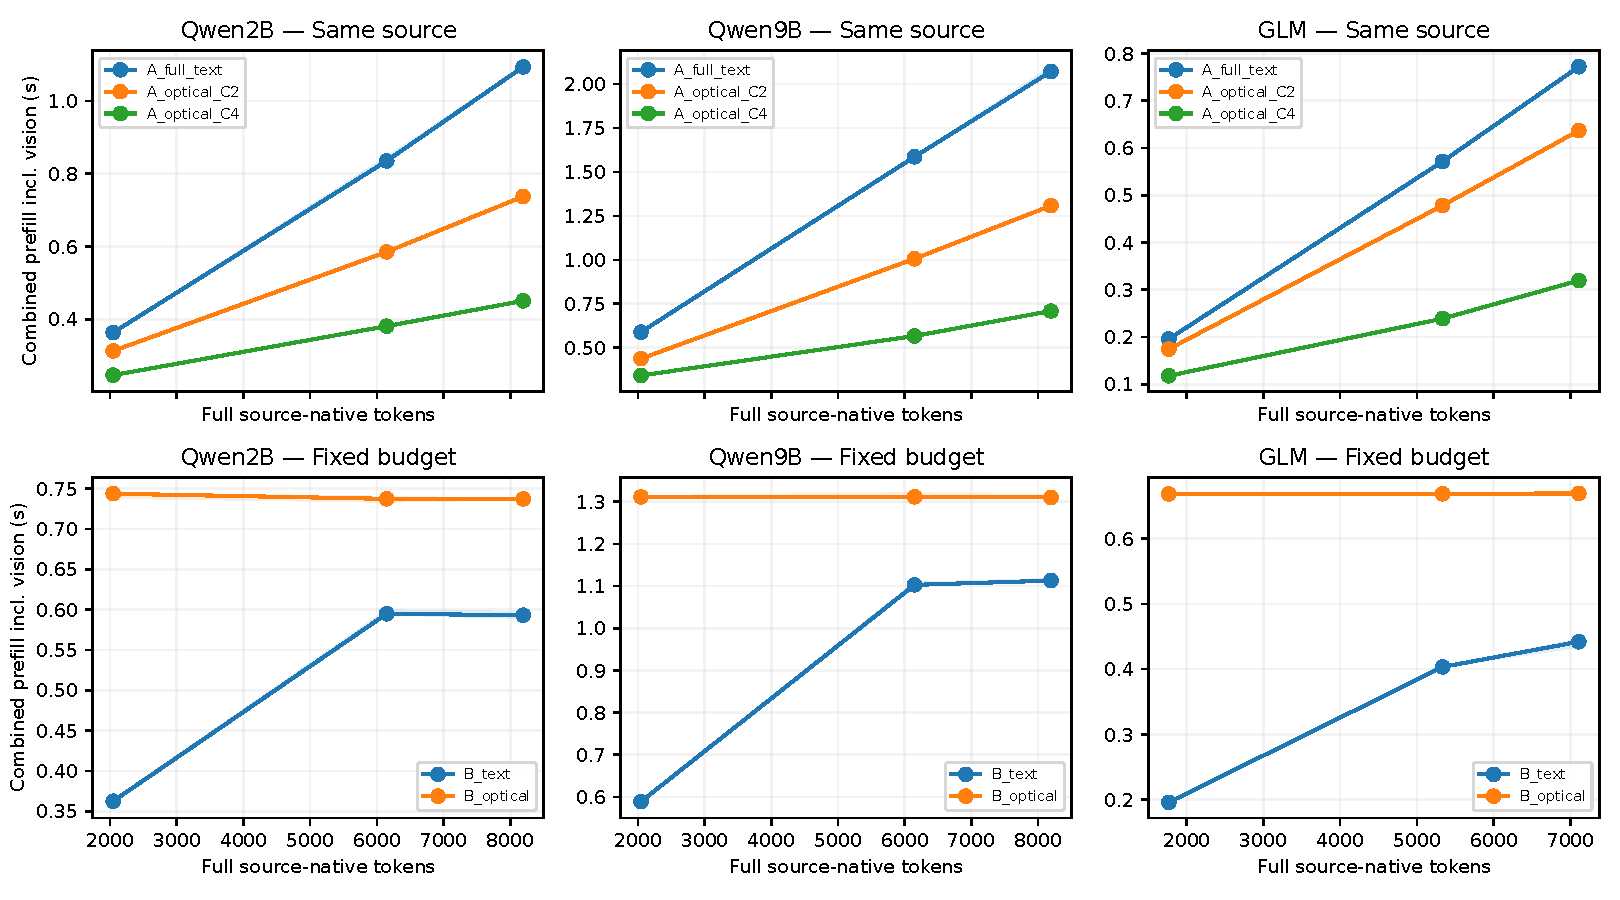
\includegraphics[width=\linewidth]{figures/systems_prefill.pdf}
\caption{Complete original audited combined-prefill profiles, with same-source and fixed-budget views distinguished. Dispersion bands show run IQRs for the predetermined case, not confidence intervals over source documents. Per-reader axes may differ.}
\end{figure}
\begin{figure}[p]\centering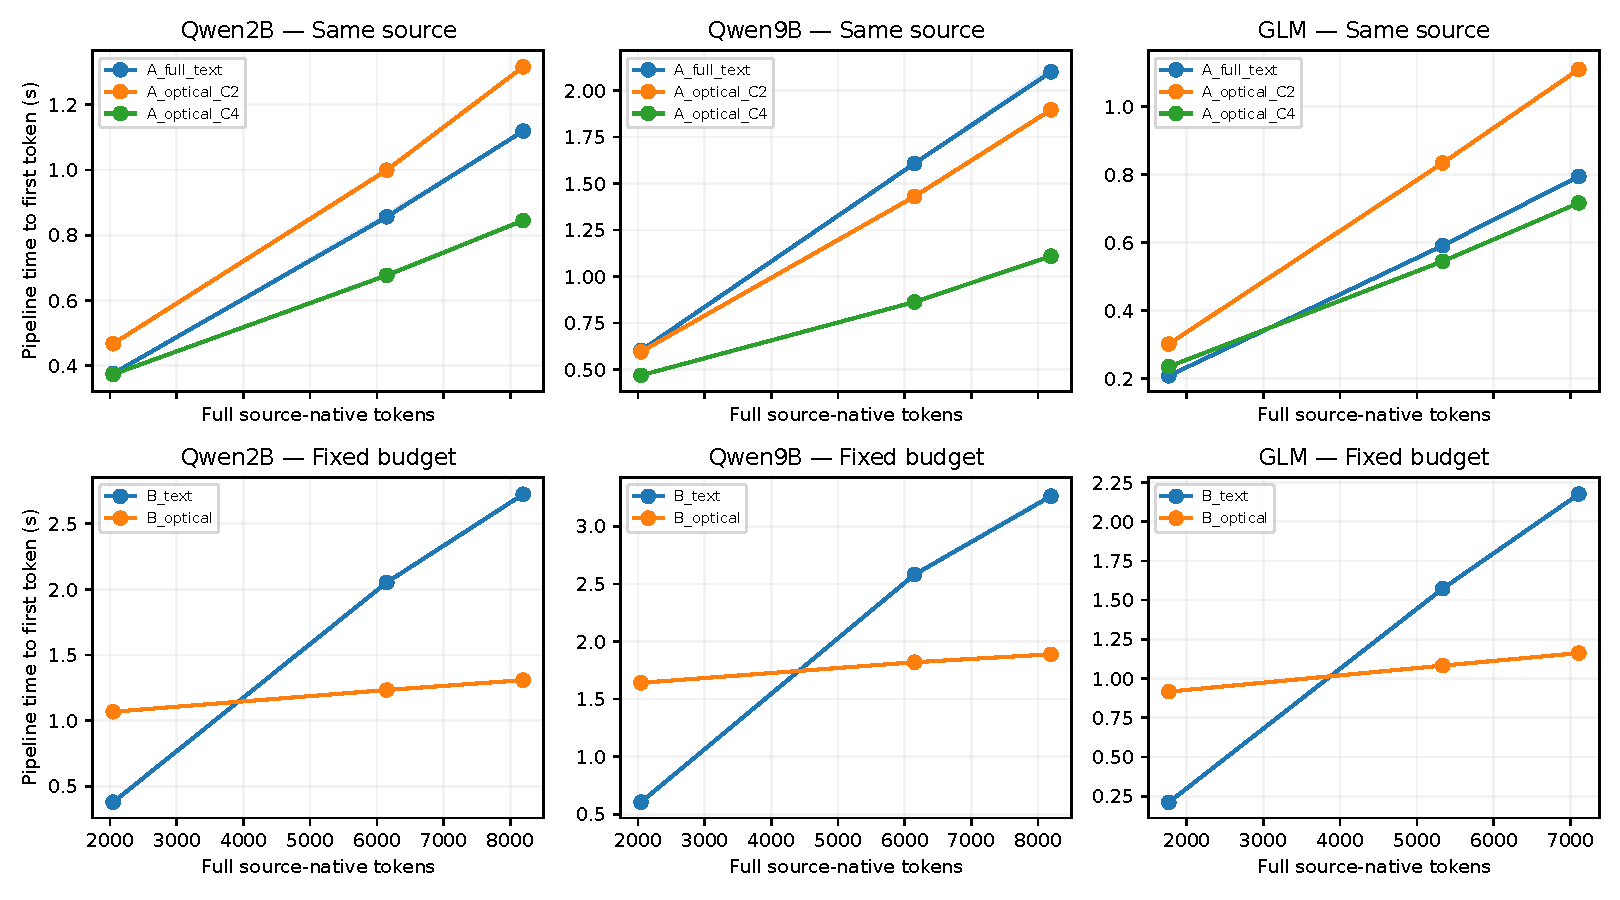
\includegraphics[width=\linewidth]{figures/systems_ttft.pdf}
\caption{Complete original audited pipeline-TTFT profiles. Pipeline TTFT includes representation preparation and processing; optical layout plans are precomputed, while retained-text packing is recomputed. This asymmetry is part of the measured implementation.}
\end{figure}
\begin{figure}[p]\centering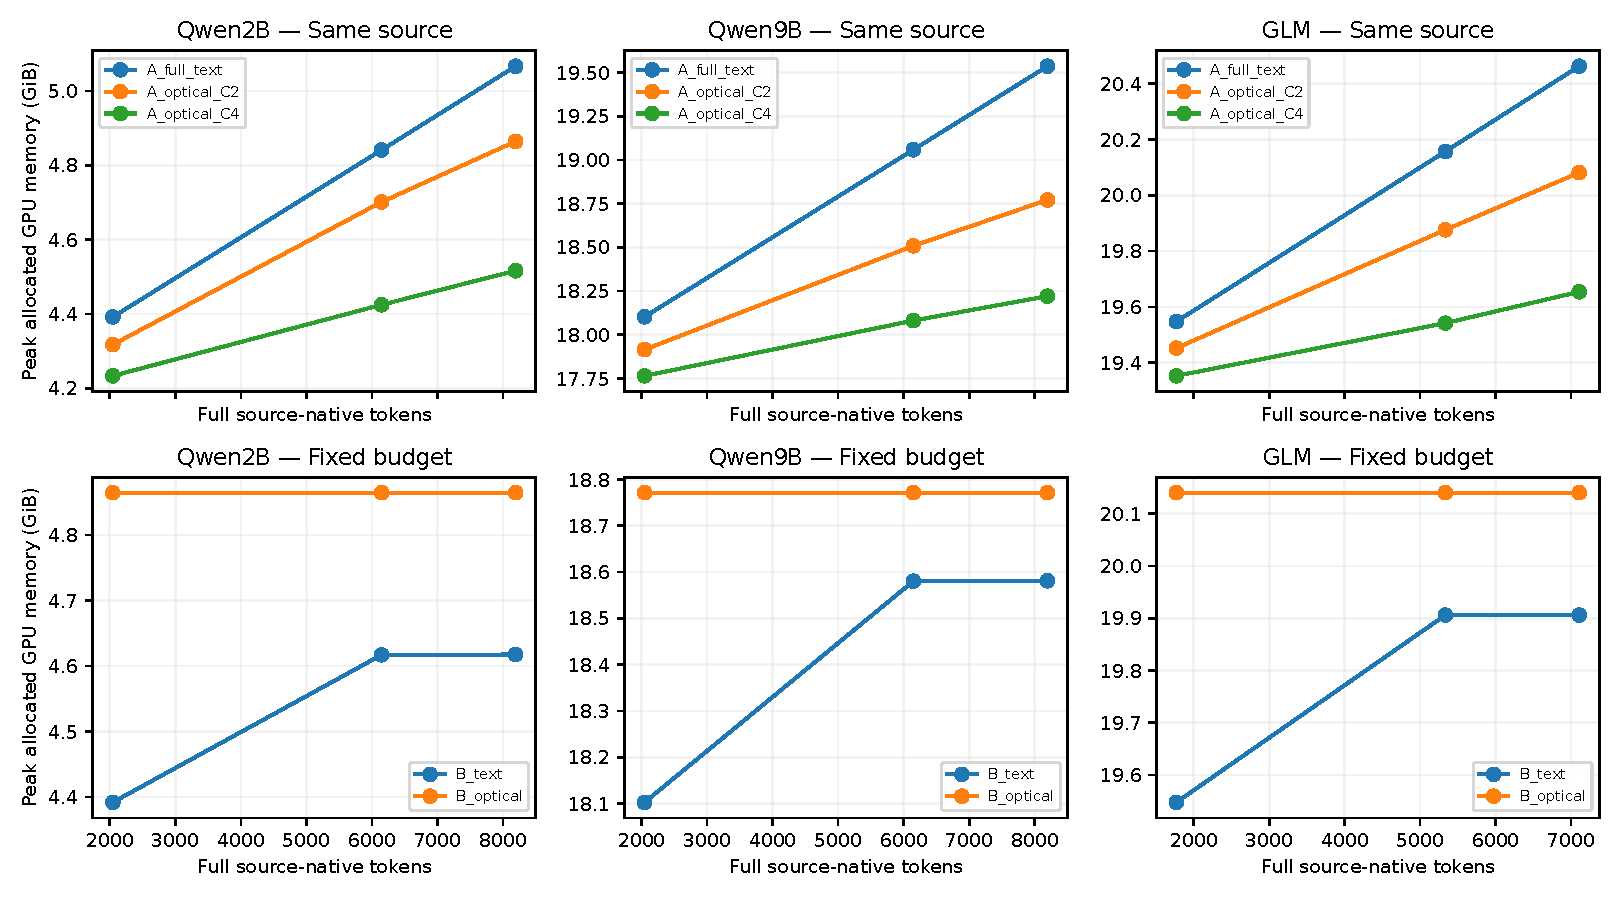
\includegraphics[width=\linewidth]{figures/systems_memory.pdf}
\caption{Complete original audited peak allocated-memory profiles. Resident model allocation is included. Per-panel scales can differ and need not start at zero; numerical differences should guide comparisons.}
\end{figure}
\clearpage
